\chapter{Un \textit{wearable device} pour la reconnaissance des sols}
\label{chap:4}

Dans le chapitre précédent, les différentes technologies aussi bien matérielles que logicielles qui sont utilisées dans la conception des \textit{wearable devices} ont été présentées. Puisque ces technologies sont nombreuses, il demeure donc important de bien cibler celles qui doivent être utilisées afin que la conception des \textit{wearable devices} réponde à la problématique exprimée. Ainsi, la principale question qui est traitée dans ce chapitre est : \textit{\og quels sont les nouveaux apports, en matière d'Intelligence Ambiante, que les wearable devices vont permettre de proposer aux résidents des habitats intelligents afin d'améliorer l'assistance qui leur est requise ? \fg}.

Pour répondre à cette question, notre travail s'est concentré sur un exemple précis d'utilisation des \textit{wearable devices} : la reconnaissance des différents types de sols à l'aide de données inertielles produites par la démarche humaine. Ce cas d'application est directement lié à la problématique générale de l'assistance, car au sein des habitats intelligents, les résidents doivent constamment s'adapter à différents types de sols. Dans ce contexte, lorsqu'il s'agit de personnes en perte d'autonomie ou ayant des troubles moteurs, certains sols peuvent alors représenter des dangers ou causer de la peur chez les résidents, car il est possible que ces sols soient plus ou moins meubles ou glissants. Par exemple, il est possible de mentionner les tapis ou le carrelage mouillé dans la salle de bain.

De manière générale, très peu de travaux proposant une méthode de reconnaissance des types de sols ont été identifiés dans la littérature. Ainsi, la première partie de ce chapitre présente brièvement les méthodes qui s'appuient sur des données inertielles produites par des robots. Ensuite, après avoir présenté la solution proposée ainsi que les expérimentations réalisées, ce chapitre va analyser et discuter les résultats obtenus. Finalement, la dernière partie dresse une conclusion de ce premier travail.

\section{La problématique spécifique de la reconnaissance des types de sols}
\label{sec:rw}
Dans le domaine de la reconnaissance des types de sols, la majorité des travaux que nous avons recensés concerne des méthodes qui ont été développées pour être utilisées avec des robots. Bien que ceux-ci soient, d'une certaine manière, pertinents pour comprendre comment reconnaître différents types de sols, ces méthodes ne sont pas directement adaptées pour effectuer, de façon appropriée, une telle reconnaissance dans le contexte de la démarche humaine. Par ailleurs, la compréhension de ces travaux a permis de guider les choix de conception de la méthode et du protocole expérimental qui sont proposés dans ce chapitre.

Dans le domaine de la robotique, l'idée de reconnaître des types de sols, et plus particulièrement, par le biais de données produites par une centrale inertielle n'est pas nouvelle. Tout d'abord, \cite{Vail2004} ont expérimenté la détection de surface grâce à des données inertielles produites par un robot quadrupède. Pour réaliser l'apprentissage, les auteurs ont opté pour un algorithme dont le modèle est un arbre de décision (\texttt{C4.5}), car ils estiment qu'il s'agit d'un algorithme suffisamment rapide et facile à représenter et à implémenter. Pour quantifier la précision de leur modèle d'apprentissage, \citeauthor{Vail2004} ont utilisé la technique de la validation croisée en 10-plis \citep{Kohavi1995}, ce qui leur a permis d'obtenir un taux de reconnaissance global de 84.9\% (ciment: 91\%; tapis: 81.2\%; champs: 81.2\%). Par la suite, \cite{Kertesz2016} a également présenté une méthode permettant de reconnaître des sols avec un accéléromètre embarqué sur un robot quadrupède. Un taux de reconnaissance de 96.2\% a été obtenu grâce à une forêt d'arbres décisionnels (\acl{RF} ou \acs{RF}), où la précision de l'apprentissage a été évaluée avec la même technique que celle utilisé par \citeauthor{Vail2004}. La différence majeure entre les deux travaux réside principalement dans le fait que les premiers ont exploité des caractéristiques temporelles du signal inertiel (variance et correlation) pour concevoir leur modèle d'apprentissage, tandis que le second a employé des caractéristiques fréquentielles obtenues grâce à une \acs{FFT}.

Par ailleurs, \cite{Bibuli2007} ont proposé une méthode de reconnaissance des sols pour un robot à quatre roues équipé de plusieurs types de capteurs, dont une centrale inertielle. Pour ce faire, ils ont tout d'abord calculé les composantes fréquentielles du signal inertiel \textit{via} l'algorithme de la transformée de Fourrier discrète (\acl{DFT} ou \acs{DFT}), pour chacun des axes du capteur. Ensuite, chaque ensemble de données résultant de cette transformation a été entraîné distinctement par un réseau de neurones artificiels (\acs{ANN}). Par conséquent, les meilleurs résultats ont été obtenus avec les données de l'axe $x$ du gyroscope, soit respectivement 90\%, 71.2\%, 70\%, 98.8\% et 83.5\% pour les sols en graviers, gazon, sable, pavés et terre.

Enfin, \cite{Weiss2007} ont proposé une comparaison de plusieurs méthodes pour réaliser une reconnaissance de sols avec un robot à quatre roues doté d'un capteur inertiel. Plus précisément, ils ont comparé l'algorithme \acs{SVM} avec d'autres types d'algorithmes d'apprentissage où les données fournies en entrée sont des caractéristiques fréquentielles du signal inertiel correspondant à différentes vitesses du robot (0.2, 0.4 et 0.6 m/s) et pour six sols distincts (sol intérieur, asphalte, gravier, gazon, pavés, sol argileux). Avec l'obtention de 77\% de taux de confiance, leur étude a montré de meilleurs résultats avec l'algorithme \acs{SVM} qu'avec les autres algorithmes qui sont : un réseau de neurones probabiliste (\acl{PNN} ou \acs{PNN}), l'algorithme des $k$ plus proches voisins, l'algorithme bayésien naïf et \texttt{C4.5}.

Au mieux de notre connaissance, il apparait que peu de recherches ont été proposées pour exploiter une telle reconnaissance avec l'humain. Pourtant, de nombreux cas d'utilisation à la reconnaissance des sols dans ce contexte nous paraissent exploitables. En effet, dans l'objectif de proposer une meilleure assistance aux résidents des habitats intelligents, il semble important d'apporter des réponses à cette problématique spécifique. Par exemple, des techniques de prévention des chutes plus efficaces permettraient alors de rassurer et d'aider les personnes en perte d'autonomie ou ayant des troubles moteurs lors de leur évolution au sein de ce genre d'habitats.

De ce fait, \cite{Otis2016}, au travers de leurs travaux sur la stimulation vibrotactile pour la réduction des risques de chutes, ont proposé une méthode basée sur la reconnaissance des types de sols. Pour ce faire, une chaussure embarquant un accéléromètre a été fabriquée. Ensuite, un algorithme de \textit{clustering} a été utilisé pour segmenter les caractéristiques fréquentielles discriminantes obtenues par le biais de la \acs{FFT} sur le signal accéléromètrique lorsque celui-ci a été enregistré sur les sols suivants : gravier, ciment, sable, neige et glace. En ce qui concerne les résultats obtenus, les auteurs mentionnent un taux d'erreurs compris entre 1\% et 5\% lors des essais en laboratoire, alors qu'ils ont observé une augmentation de ce taux en conditions réelles, soit 20\% d'erreurs. Malgré l'absence de détails supplémentaires sur l'obtention de ces résultats, le travail réalisé par \cite{Otis2016} nous a permis d'identifier un protocole expérimental adapté à mettre en \oe{}uvre. Ceci dans le but d'être le plus fidèle aux conditions réelles d'utilisation, ainsi que pour faciliter la comparaison de la méthode proposée dans ce chapitre avec de futures implémentations.

\section{Solution proposée}

\subsection{Le \textit{wearable device}}

Selon la littérature existante, l'utilisation de centrales inertielles pour réaliser la reconnaissance de sols s'est révélée être une technique aussi bien fonctionnelle avec des robots qu'avec les individus. De ce fait, la contribution présentée dans ce chapitre s'est, dans un premier temps, axée sur la conception d'un \textit{wearable device} pour y parvenir. L'idée générale est de piloter, par l'intermédiaire d'un téléphone connecté en \acs{BLE} (\texttt{cell\_oper}), le dispositif afin d'enregistrer un volume important de données pendant une marche. Lors de la conception, le choix s'est porté sur le système sur puce (\acl{SOC} ou \acs{SOC}) \textit{Arduino 101} qui embarque le module \textit{Intel Curie}, également accompagné d'un \textit{shield} de prototypage sur lequel est embarqué un lecteur de carte mémoire, tel qu'illustré en figure \ref{fig:device}. Ce choix a été motivé par la composition même du module \textit{Intel Curie}. En effet, ce dernier intègre d'usine un module de communication \acs{BLE}, un \acs{IMU} 6-axes (6-\acl{DOF} ou 6-\acs{DOF}) ainsi qu'une quantité suffisante d'Entrées/Sorties (\acl{IO} ou \acs{IO}) pour connecter des composants supplémentaires et ainsi faciliter l'évolution du dispositif. De plus, les autres avantages au choix de ce matériel demeurent la simplicité et la fiabilité de l'\textit{Arduino 101}, mais également la quantité de ressources disponibles pour cette plateforme \hl{(librairies, pilotes, \textit{etc.})}. Finalement, la présence d'un lecteur de carte mémoire sur le \textit{shield} de prototypage constitue un moyen simple et efficace pour gérer la quantité de données inertielles qui doivent être stockées.

\begin{figure}[H]
	\centering
	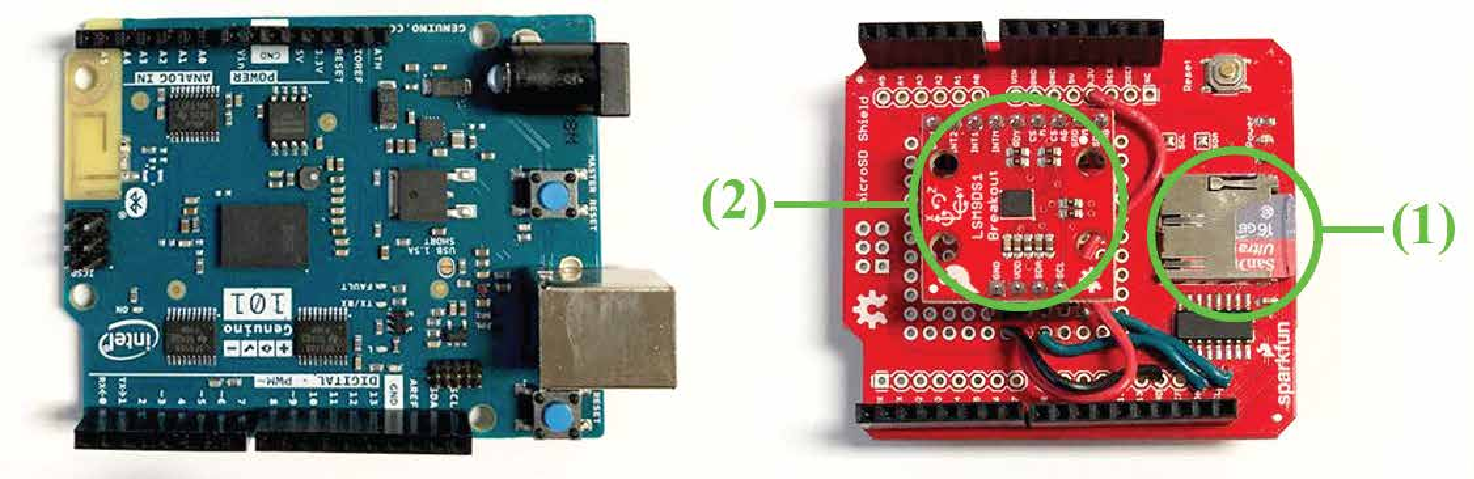
\includegraphics[width=.8\linewidth]{chapter4/device.pdf}
        \caption[\acs{SOC} Arduino 101 et son \textit{shield} de prototypage incluant une carte mémoire (1) ainsi que la centrale inertielle \textit{LSM9DS1} (2) présente sur la version 2 du dispositif.]{\acs{SOC} Arduino 101 et son \textit{shield} de prototypage incluant une carte mémoire (1) ainsi que la centrale inertielle \textit{LSM9DS1} (2) présente sur la version 2 du dispositif \citep{Thullier2017}.}
	\label{fig:device}
\end{figure}

Dans une première version, la reconnaissance des types de sols a été réalisée par l'intermédiaire de l'IMU 6-axes directement embarqué sur le \acs{SOC} \textit{Arduino}. Néanmoins, puisque la précision de celui-ci était inconnue avant les premières expérimentations et qu'il manquait les trois axes supplémentaires du magnétomètre, une seconde version du \textit{wearable device} a été proposée. Pour cette dernière, un nouvel IMU 9-axes, le \texttt{LSM9DS1}, a été interfacé directement sur le \textit{shield} de prototypage.

\subsection{Le \textit{firmware}}

Pour assurer le bon fonctionnement du matériel qui compose le \textit{wearable device}, il était tout d'abord nécessaire de développer un \textit{firmware} \footnote{\url{https://github.com/FlorentinTh/SoilTypesRecognition-WearableFirmware}}. Le fonctionnement de celui-ci s'articule autour de trois composants logiciels principaux qui sont illustrés en figure \ref{fig:soil_types_firmware}.

\begin{figure}[H]
	\centering
	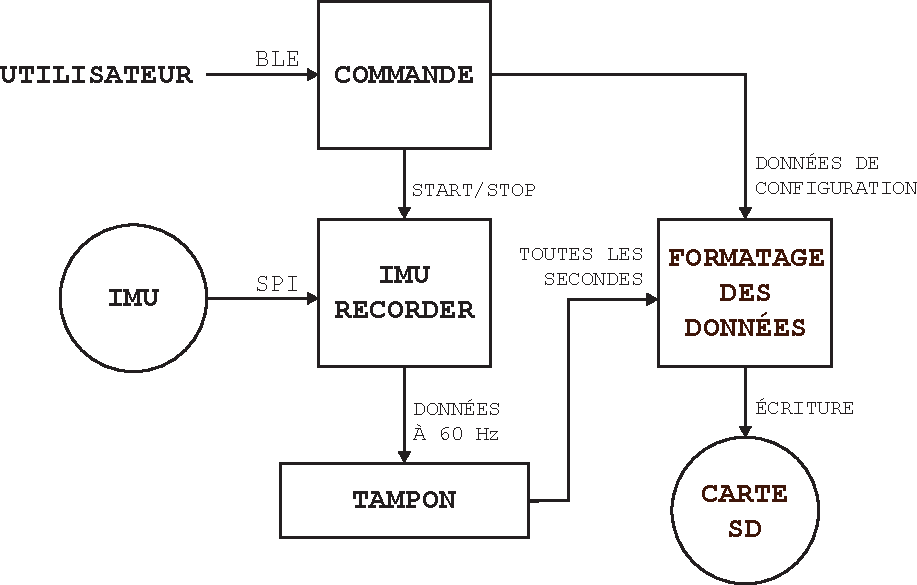
\includegraphics[width=12cm]{chapter4/soil_types_firmware.pdf}
        \caption[Implémentation du \textit{firmware} embarqué sur le \textit{wearable device}.]{Implémentation du \textit{firmware} embarqué sur le \textit{wearable device} \citep{Thullier2017}.}
	\label{fig:soil_types_firmware}
\end{figure}

Le premier est le module de \texttt{commande}. Il est en charge des communications entre le téléphone (\texttt{cell\_oper}) et le \textit{wearable device}, par l'intermédiaire du module radio \acs{BLE}. Ainsi, un téléphone ou n'importe quel autre dispositif compatible avec la technologie \acs{BLE} peut être utilisé pour étiqueter les ensembles de données enregistrés avec les informations de configuration requises (le type de sol, l'identifiant anonyme du participant et l'emplacement du dispositif). Le second module principal est l'\texttt{\acs{IMU} Recorder}. En fonction de la version du dispositif, il a pour rôle de stocker dans une mémoire tampon les valeurs de l'\acs{IMU} qui transitent soit par un bus de données \ac{SPI} dans sa première version, soit \textit{via} un bus de données \ac{I2C}, à une fréquence stabilisée à 60 Hz. Le contenu de la mémoire tampon est ensuite envoyé au module de \texttt{formatage des données} toutes les secondes. Finalement, ce composant récupère l'ensemble des données de configuration du module de commande et s'occupe d'écrire les nouvelles données dans un fichier \ac{CSV} qui est stocké sur la carte mémoire. Dans la seconde version du \textit{wearable device}, le module de \texttt{formatage des données} s'occupe également de calculer les angles d'Euler (précession, nutation et rotation propre) grâce aux trois axes supplémentaires fournis par le \texttt{LSM9DS1}.

% \subsection{Le processus d'apprentissage pour la reconnaissance des types de sols}
% \label{sec:learn}

\subsection{Extraction de caractéristiques}
% \subsubsection{Extraction de caractéristiques}

Après que les données aient été enregistrées sur la carte mémoire, le processus d'apprentissage pour la reconnaissance des types de sol peut alors débuter et sa première phase demeure l'extraction de caractéristiques. En ce sens, cette solution propose d'utiliser les caractéristiques temporelles et fréquentielles les plus employées dans le domaine de la reconnaissance d'activités, tel que discuté à la section \ref{sec:prel_steps} et qui sont rappelées par le tableau \ref{tab:features}.

La première opération consiste en une simple moyenne non pondérée sur chacun des axes tant \og{}physiques\fg{} des capteurs de l'\acs{IMU} (gyroscope, accéléromètre et magnétomètre) que \og{}logiques\fg{} (angles d'Euler), s'ils existent. Ensuite, la moyenne générale de chacune de ces caractéristiques est calculée pour l'ensemble des axes. De la même manière, cette procédure a été appliquée à plusieurs autres calculs statistiques : l'écart type, l'asymétrie (équation \ref{eq:asymetrie}), l'aplatissement (équation \ref{eq:kurtosis}), le \textit{Zero Crossing Rate} et la corrélation entre toutes les combinaisons possibles d'axes par capteurs de l'\acs{IMU} (équation \ref{eq:correlation}). Dans un second temps, une transformation du domaine temporel vers le domaine fréquentiel a été nécessaire pour obtenir les caractéristiques suivantes : la composante continue, l'énergie spectrale (équation \ref{eq:energy_spec}) et l'entropie  (équation \ref{eq:entropy}). Ce passage d'un domaine à l'autre a été réalisé en utilisant la transformation de Fourier rapide (\acs{FFT}) selon l'algorithme de Bluestein \citep{Bluestein1970}. Ainsi, en fonction de la centrale inertielle exploitée (6-axes, 9-axes ou 9-axes avec les trois angles d'Euler), ce sont 70, 105 ou 140 caractéristiques qui sont calculées sur chaque fenêtre temporelle rectangulaire et non chevauchante, dont la taille est fixée à 60 secondes. La taille de la fenêtre a été déterminée par une évaluation du temps moyen nécessaire pour marcher une distance de $4.3$ m, ce qui correspond à un aller-retour dans le bac utilisé lors des expérimentations et dont le protocole est décrit à la section \ref{sec:expe}.

\begin{table}[H]
	\caption{Récapitulatif de toutes les caractéristiques utilisées par la solution proposée en fonction du nombre d'axes offerts par la centrale inertielle.}
	\label{tab:features}
	\resizebox{\textwidth}{!}{%
	\begin{tabular}{|r|c|c|c|c|c|c|c|}
	\hline
	\multicolumn{4}{|c|}{\textbf{Domaine Temporel}} & \multicolumn{4}{c|}{\textbf{Domaine Fréquentiel}} \\ \hline
	\multicolumn{1}{|c|}{\multirow{3}{*}{\textit{\textbf{Caractéristique}}}} & \multicolumn{3}{c|}{\textit{\textbf{\begin{tabular}[c]{@{}c@{}}Nb. Total de\\[-15pt] Caractéristiques\end{tabular}}}} & \multirow{3}{*}{\textit{\textbf{Caractéristique}}} & \multicolumn{3}{c|}{\textit{\textbf{\begin{tabular}[c]{@{}c@{}}Nb. Total de\\[-15pt] Caractéristiques\end{tabular}}}} \\ \cline{2-4} \cline{6-8}
	\multicolumn{1}{|c|}{} & \textit{\begin{tabular}[c]{@{}c@{}}IMU \\[-15pt] 6 axes\end{tabular}} & \textit{\begin{tabular}[c]{@{}c@{}}IMU \\[-15pt] 9 axes\end{tabular}} & \textit{\begin{tabular}[c]{@{}c@{}}IMU \\[-15pt] 9 axes\\[-15pt] avec angles\\[-15pt] d'Euler\end{tabular}} &  & \textit{\begin{tabular}[c]{@{}c@{}}IMU \\[-15pt] 6 axes\end{tabular}} & \textit{\begin{tabular}[c]{@{}c@{}}IMU \\[-15pt] 9 axes\end{tabular}} & \textit{\begin{tabular}[c]{@{}c@{}}IMU \\[-15pt] 9 axes\\[-15pt] avec angles\\[-15pt] d'Euler\end{tabular}} \\ \hline
	Moyenne pour chaque axe & 6 & 9 & 12 & \multicolumn{1}{r|}{Composante continue pour chaque axe} & 6 & 9 & 12 \\ \hline
	Moyenne de tous les axes & 2 & 3 & 4 & \multicolumn{1}{r|}{\begin{tabular}[c]{@{}r@{}}Énergie spectrale pour chaque axe\\[-15pt] (équation \ref{eq:energy_spec})\end{tabular}} & 6 & 9 & 12 \\ \hline
	Écart type pour chaque axe & 6 & 9 & 12 & \multicolumn{1}{r|}{\begin{tabular}[c]{@{}r@{}}Entropie pour chaque axe\\[-15pt] (équation \ref{eq:entropy})\end{tabular}} & 6 & 9 & 12 \\ \hline
	Écart type pour tous les axes & 2 & 3 & 4 & - & - & - & - \\ \hline
	\begin{tabular}[c]{@{}r@{}}Asymétrie pour chaque axe\\[-15pt] (équation \ref{eq:asymetrie})\end{tabular} & 6 & 9 & 12 & - & - & - & - \\ \hline
	Asymétrie pour tous les axes & 2 & 3 & 4 & - & - & - & - \\ \hline
	\begin{tabular}[c]{@{}r@{}}Aplatissement pour chaque axe\\[-15pt] (équation \ref{eq:kurtosis})\end{tabular} & 6 & 9 & 12 & - & - & - & - \\ \hline
	Aplatissement pour tous les axes & 2 & 3 & 4 & - & - & - & - \\ \hline
	\begin{tabular}[c]{@{}r@{}}Corrélation entre toutes les combinaisons \\[-15pt] possibles d'axes incluant le total des axes\end{tabular} & 12 & 18 & 24 & - & - & - & - \\ \hline
	Zero Crossing Rate pour chaque axe & 6 & 9 & 12 & - & - & - & - \\ \hline
	Zero Crossing Rate pour tous les axes & 2 & 3 & 4 & - & - & - & - \\ \hline
	\textit{\textbf{Sous-total}} & \textit{\textbf{52}} & \textit{\textbf{78}} & \textit{\textbf{104}} & \multicolumn{1}{r|}{\textit{\textbf{Sous-total}}} & \textit{\textbf{18}} & \textit{\textbf{27}} & \textit{\textbf{36}} \\ \hline
	\multirow{4}{*}{\textbf{Total}} & \multicolumn{1}{r|}{\textit{\textbf{\begin{tabular}[c]{@{}r@{}}IMU\\[-15pt] 6 axes\end{tabular}}}} & \multicolumn{6}{c|}{\textbf{70}} \\ \cline{2-8}
	 & \multicolumn{1}{r|}{\textbf{\begin{tabular}[c]{@{}r@{}}IMU\\[-15pt] 9 axes\end{tabular}}} & \multicolumn{6}{c|}{\textbf{105}} \\ \cline{2-8}
	 & \multicolumn{1}{r|}{\textbf{\begin{tabular}[c]{@{}r@{}}IMU 9 axes\\[-15pt] avec angles d'Euler\end{tabular}}} & \multicolumn{6}{c|}{\textbf{140}} \\ \hline
	\end{tabular}%
	}
\end{table}

% \subsubsection{Apprentissage}

Dès l'obtention des caractéristiques discriminantes, l'étape suivante requise pour réaliser la reconnaissance des sols est le processus d'apprentissage. Selon la littérature qui concerne la reconnaissance d'activités, mais également celle au sujet de la reconnaissance des sols en robotique qui ont été respectivement discutées dans les sections \ref{sec:algos} et \ref{sec:rw}, la performance de plusieurs algorithmes d'apprentissage a pu être démontrée. Néanmoins, ce premier travail propose une comparaison entre deux algorithmes qui n'ont pas encore été présentés dans cette thèse : la forêt d'arbres décisionnels (\textit{random forest}) et les $k$ plus proches voisins (\acl{KNN} ou \acs{KNN}). Ce choix est motivé par deux raisons principales. La première est que ces deux techniques d'apprentissage appartiennent à deux familles distinctes\textemdash respectivement, les arbres de décision et les algorithmes d'apprentissage \og{}paresseux\fg{}. De plus, ceux-ci constituent tous deux des méthodes non paramétriques, c'est-à-dire, qui ne font aucune supposition quant à la distribution de l'échantillon de données fournies en entrée. De ce fait, ces méthodes demeurent simples, flexibles et efficaces \citep{Russell2010}. Par ailleurs, la performance en termes de taux de reconnaissance obtenue avec ces algorithmes est souvent exposée dans la littérature \citep{Kertesz2016, Vail2004}.

\subsection{l'algorithme \textit{random forest}}

Selon \cite{Breiman2001}, une forêt d'arbres décisionnels est une combinaison d'arbres prédicteurs, aussi appelés arbre de décision, où chacun d'eux dépend d'un vecteur de données distinct, mais de même cardinalité. Ce vecteur contient un sous-ensemble aléatoire des données initiales issues de la phase d'extraction des caractéristiques. La décision finale du processus de reconnaissance de cet algorithme est déterminée par un vote majoritaire entre chacune des décisions émises en sortie des arbres de décision qui composent la forêt. La figure \ref{fig:algo_random_forest} illustre un exemple simplifié d'une forêt d'arbres décisionnels utilisant trois arbres.

\begin{figure}[H]
	\centering
	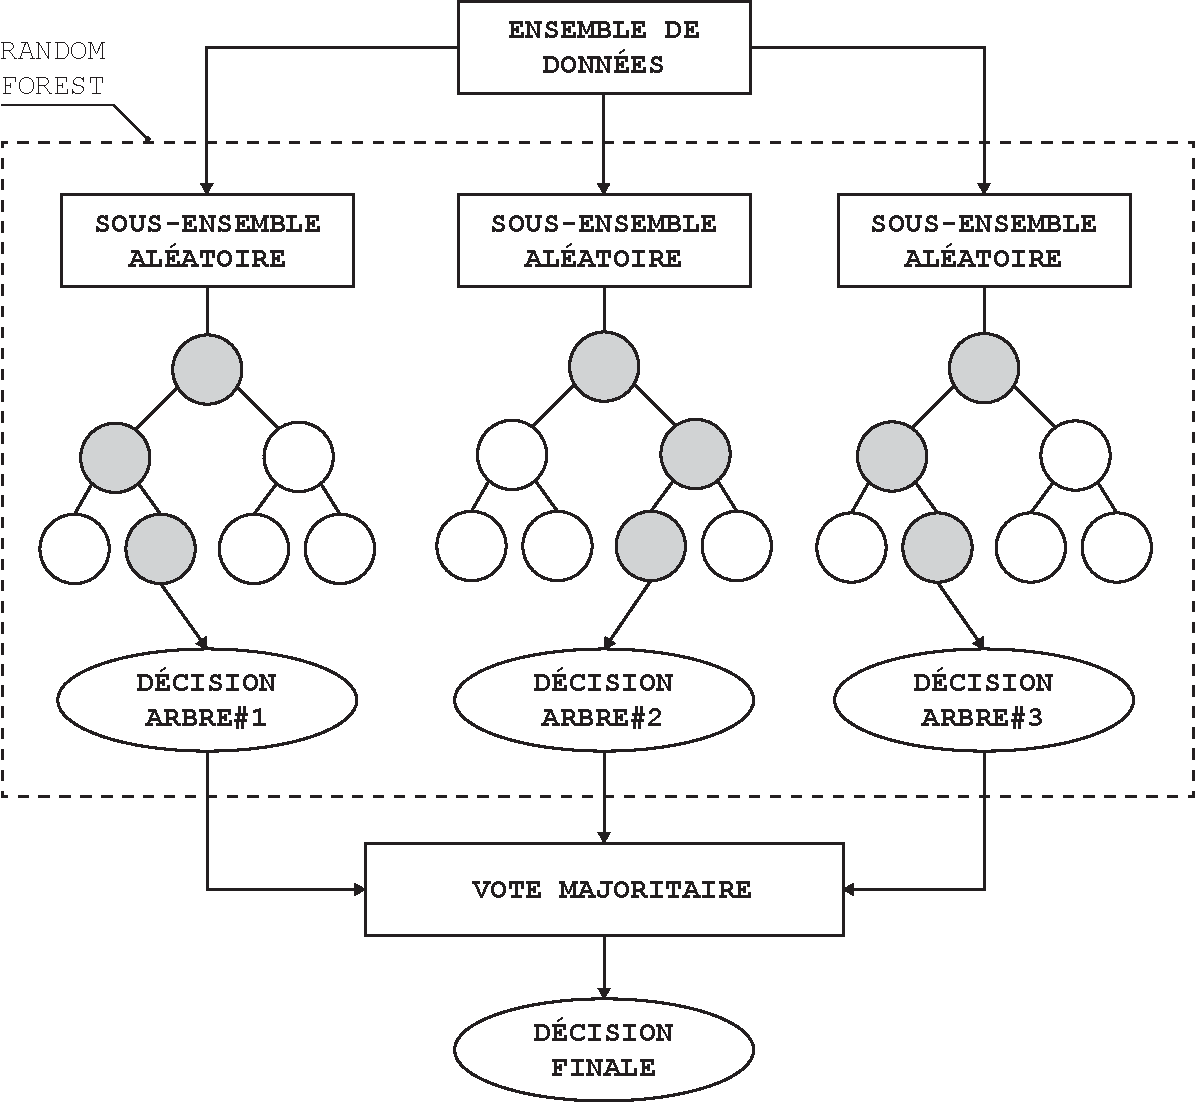
\includegraphics[width=.7\linewidth]{chapter4/algo_random_forest.pdf}
  \caption[Exemple de l'algorithme \textit{random forest} utilisant $B=3$ arbres.]{Exemple de l'algorithme \textit{random forest} utilisant $B=3$ arbres \citep{Thullier2017}.}
	\label{fig:algo_random_forest}
\end{figure}

Pour exploiter la forêt d'arbres décisionnels en tant qu'algorithme d'apprentissage, il est important de définir préalablement au moins trois paramètres principaux. Le premier est le nombre d'arbres que doit comporter la forêt ($B$). Le second correspond au nombre de caractéristiques à considérer dans la division des n\oe{}uds de l'arbre lors de la construction de ce dernier ($F$) et enfin, la fonction nécessaire à la mesure de la qualité de cette division ($C$). En ce qui concerne le nombre de caractéristiques, \citeauthor{Breiman2001} suggère d'utiliser $F_1=\lfloor log_2(m) + 1\rfloor$ où $m$ fait référence au nombre total d'attributs présents dans le jeu de données fourni en entrée. Néanmoins, il est également possible de trouver d'autres recommandations comme $F_0=\lfloor \frac{1}{2}\sqrt{m}\rfloor$ ou encore $F_2=\lfloor \sqrt{m}\rfloor$. Par ailleurs, en ce qui concerne la mesure de la qualité de la division des n\oe{}uds, les fonctions qui sont les plus couramment utilisées sont le calcul du c\oe{}fficient de Gini et l'évaluation du gain en information basé sur l'entropie de Shannon ($E$) dont les équations sont respectivement rappelées ci-après :

\begin{equation}
	\label{eq:gini}
	Gini(T) = {1-\sum_{i=1}^{n}(p_i)}^2
\end{equation}

\begin{equation}
	\label{eq:gain}
	E(T) = \sum_{i=1}^{n}-(p_i log_2 p_i)
\end{equation}

\noindent où $T$ correspond aux données qui contiennent les instances de $n$ étiquettes et $p_i$ est la fréquence relative de l'étiquette $i \in n$ dans $T$. Le choix quant à ce paramètre dépend essentiellement du type d'arbre de décision qui est utilisé lors de la construction de la forêt (\textit{p. ex.} ID3, \texttt{C4.5}, CART, \textit{etc.}).

\subsection{l'algorithme des $k$ plus proches voisins}

D'autre part, l'algorithme des $k$ plus proches voisins est considéré comme une technique d'apprentissage dite \og{}paresseuse\fg{}, ce qui veut dire qu'il n'admet pas de phase d'entraînement, ou que celle-ci demeure minime. Bien que cet algorithme soit relativement rapide et flexible, la décision finale d'étiquetage est réalisée en se basant sur l'intégralité du jeu de données utilisé pour l'entraînement. En conséquence, celui-ci doit être stocké en mémoire, ce qui implique alors la nécessité de disposer d'une quantité de stockage importante. En effet, cette méthode suppose que les données peuvent être représentées dans un espace vectoriel de caractéristiques qui peut être multidimensionnel. Ainsi, la phase d'apprentissage de l'algorithme consiste à stocker les vecteurs de données ainsi que les étiquettes qui leur sont associés. Ensuite, lors de la phase de reconnaissance, il s'agit de déterminer quels sont les $k$ vecteurs de caractéristiques qui sont les plus proches pour chaque nouvelle donnée à étiqueter, où $k$ est un paramètre qui doit être défini préalablement. Ces plus proches voisins sont alors extraits grâce à une fonction de mesure qui doit également être déterminée au préalable (\textit{p. ex.} la distance euclidienne : $D_e$ ou la distance de Manhattan : $D_m$ respectivement données en équations \ref{eq:dist_euclidean} et \ref{eq:dist_manhattan}). Finalement, l'étiquette de la nouvelle donnée est alors attribuée selon un vote majoritaire entre celles de chaque $k$ plus proche voisin. \hl{Ce fonctionnement décrit la méthode de recherche des plus proches voisins dite linéaire. Elle demeure la plus couramment utilisée bien qu'il existe d'autres possibilités comme \textit{KD-Tree} ou \textit{Ball-Tree}} \citep{Bhatia2010} \hl{permettant d'optimiser cette opération de recherche, tant en termes de rapidité d'exécution que de consommation d'espace mémoire.} La figure \ref{fig:algo_knn} illustre un exemple de cette méthode d'apprentissage avec $k=3$ plus proches voisins.

\begin{figure}[H]
	\centering
	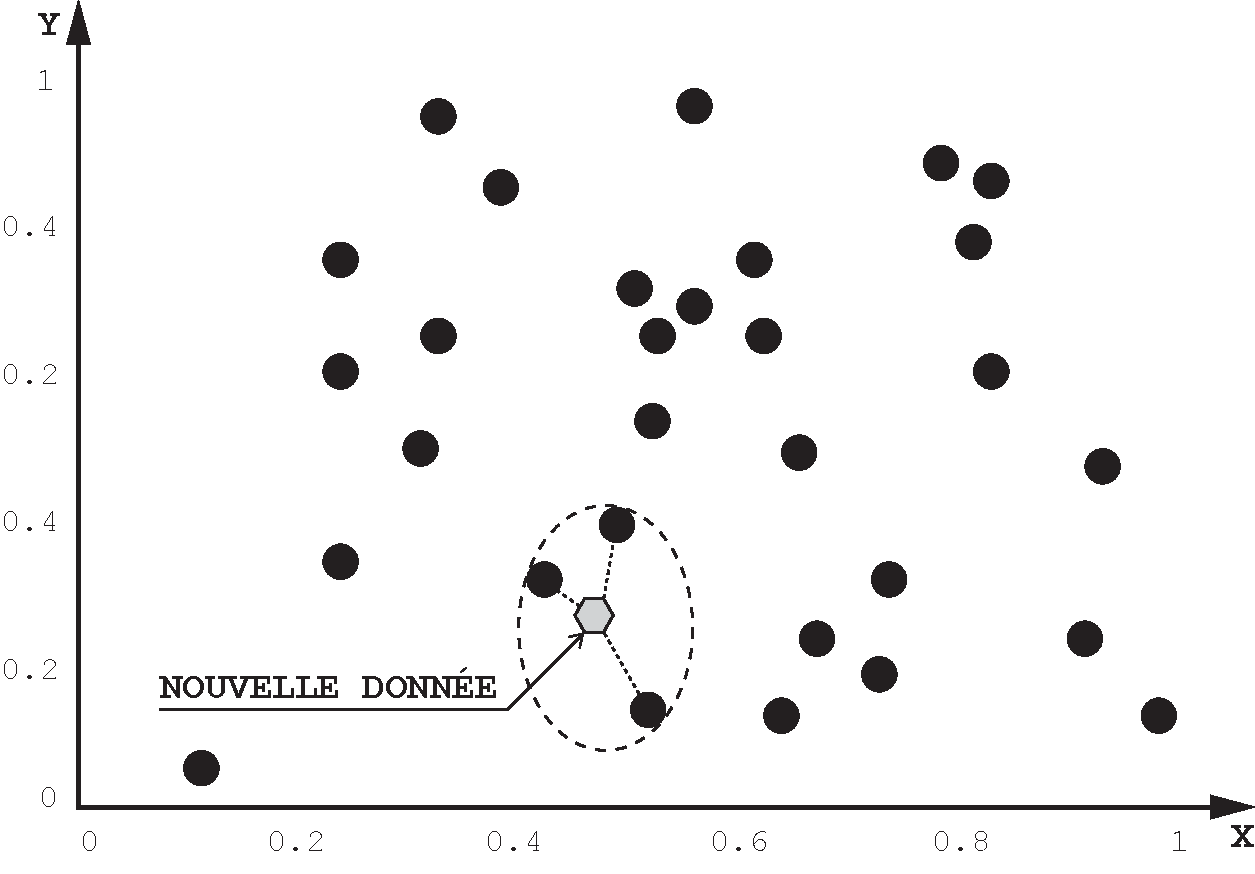
\includegraphics[width=.55\linewidth]{chapter4/algo_knn.pdf}
        \caption[Exemple de l'algorithme des $k$ plus proches voisins où $k=3$.]{Exemple de l'algorithme des $k$ plus proches voisins où $k=3$ \citep{Thullier2017}.}
	\label{fig:algo_knn}
\end{figure}

\section{Expérimentations}
\label{sec:expe}

Les expérimentations mises en place pour valider le système de reconnaissance des sols se sont déroulées en deux étapes et à deux périodes de l'année différentes. La première a été réalisée en hiver, avec la première version du \textit{wearable device} : \texttt{wear\_v1}. Elle a impliqué neuf étudiants universitaires, tous des hommes ayant entre 22 et 36 ans. Leurs poids se situaient entre $65\:kg$ et $110\:kg$ (poids médian : $80\:kg$) et leurs tailles étaient comprises entre $172\:cm$ et $192\:cm$ (taille médiane : $183\:cm$). Parmi ceux-ci, il y avait 7 droitiers pour 2 gauchers et tous étaient en bonne santé sans aucun problème de motricité. La seconde étape, quant à elle, s'est déroulée en été avec la deuxième version du dispositif : \texttt{wear\_v2} et un téléphone intelligent : \texttt{cell} (\textit{Huawei Nexus 6P} avec la version $8.0$ d'\textit{Android}). Cependant, seulement six participants sur les neuf de la première étape ont été en mesure de mener à bien cette seconde expérimentation en raison de la fin de leur cursus universitaire. Par ailleurs, notre protocole expérimental a fait intervenir des types de sols qui, bien que peu représentatifs pour le contexte de l'assistance dans les habitats intelligents, demeurent suffisamment discriminants pour, dans un premier temps, valider la faisabilité d'une telle méthode.

\subsection{Mise en \oe{}uvre}

Dans un premier temps, puisque l'\acs{UQAC} se situe dans une région où les conditions météorologiques peuvent être difficiles, la plupart des différents types de sols sont, en fonction de la période de l'année, recouverts de glace ou de neige. Pour remédier à cette problématique, un bac a été fabriqué afin d'assurer le déroulement des expérimentations à l'intérieur du laboratoire. Par conséquent, le contenu de celui-ci était soit du gravier, soit du sable, tel qu'illustré par la figure \ref{fig:box}.

\begin{figure}[H]
	\centering
	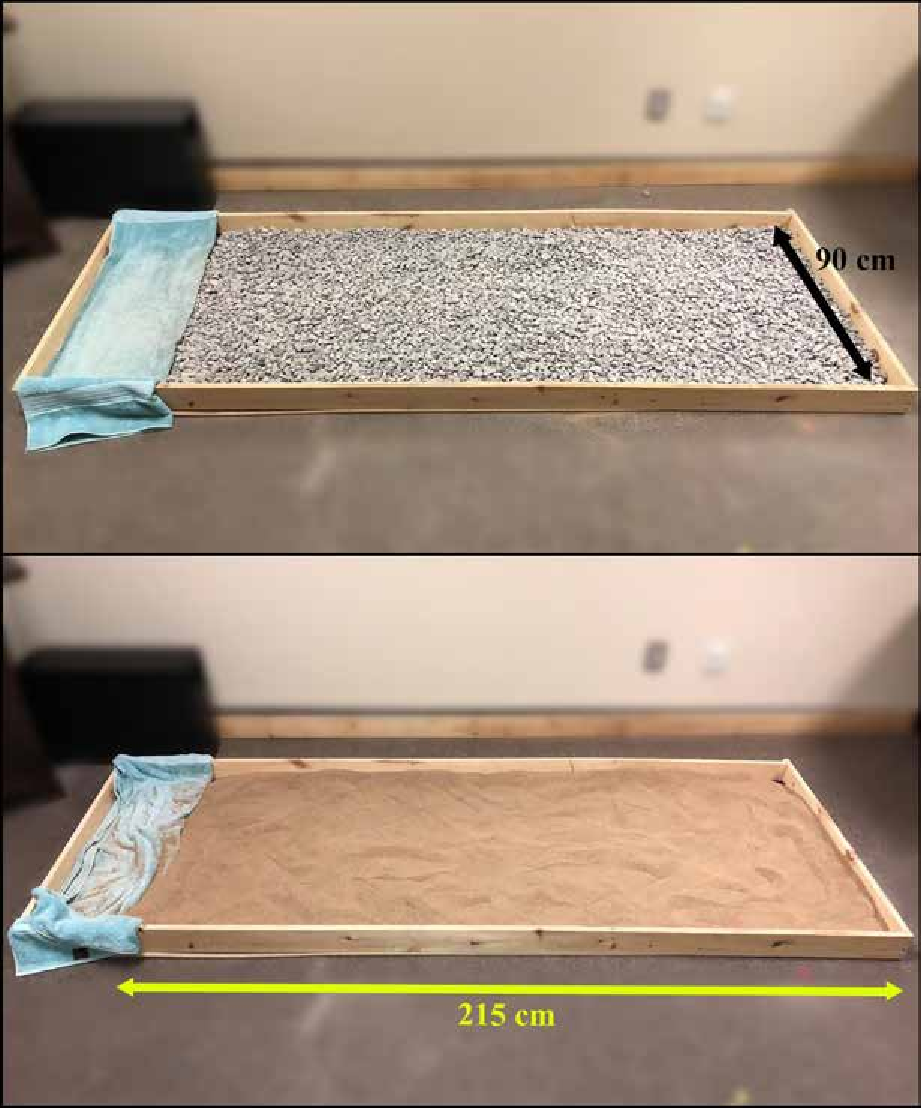
\includegraphics[width=.7\linewidth]{chapter4/box.pdf}
        \caption[Bac utilisé lors des expérimentations rempli de haut en bas, de gravier et de sable (dimensions: $l : 215\; cm \times L : 90\; cm \times H : 15\; cm$).]{Bac utilisé lors des expérimentations rempli de haut en bas, de gravier et de sable (dimensions: $l : 215\; cm \times L : 90\; cm \times H : 15\; cm$) \citep{Thullier2017}.}
	\label{fig:box}
\end{figure}

Dans un deuxième temps, une application\footnote{\url{https://github.com/FlorentinTh/SoilTypesRecognition-AndroidAppDriver}} \textit{Android} a été développée afin de piloter les expérimentations et par conséquent, étiqueter les jeux de données pour chacun des enregistrements produits par les participants. Celle-ci a permis de définir les temps de début et de fin, ainsi que les différentes informations de configuration (le type de sol, l'identifiant anonyme du participant et l'emplacement du dispositif) par le biais d'un téléphone intelligent spécifiquement dédié à cette tâche : \texttt{cell\_oper} (\textit{LG Nexus 5} avec la version $6.0.1$ d'\textit{Android}). Puisque le \textit{wearable device} est doté d'une connectivité \acs{BLE}, la première opération a consisté en un balayage afin d'obtenir la liste des appareils émetteurs aux alentours. Dans notre cas, \texttt{cell\_oper} est le dispositif périphérique et le \textit{wearable device} est le dispositif central. Ensuite, dès que les deux appareils ont été couplés, le \textit{wearable device} est alors devenu le serveur \acs{GATT} et \texttt{cell\_oper} le client, tel qu'illustré par le premier écran de la figure \ref{fig:application}. Enfin, l'enregistrement des données sur le \textit{wearable device} a débuté dès lors que les informations de configuration ont été renseignées et que le bouton d'envoi des données a été appuyé, comme le montre le second écran de la figure \ref{fig:application}.

L'avantage principal de cette méthode réside principalement dans la mobilité qu'offre l'utilisation d'un téléphone intelligent par rapport à un ordinateur traditionnel\textemdash ce qui a fortement facilité la tâche de supervision des expérimentations. De plus, l'application a pu être réutilisée sans subir de modifications aussi bien avec les deux versions du \textit{wearable device} (\texttt{wear\_v1} et \texttt{wear\_v2}) qu'avec le téléphone intelligent utilisé pour l'enregistrement de données (\texttt{cell}).

\begin{figure}[H]
	\centering
	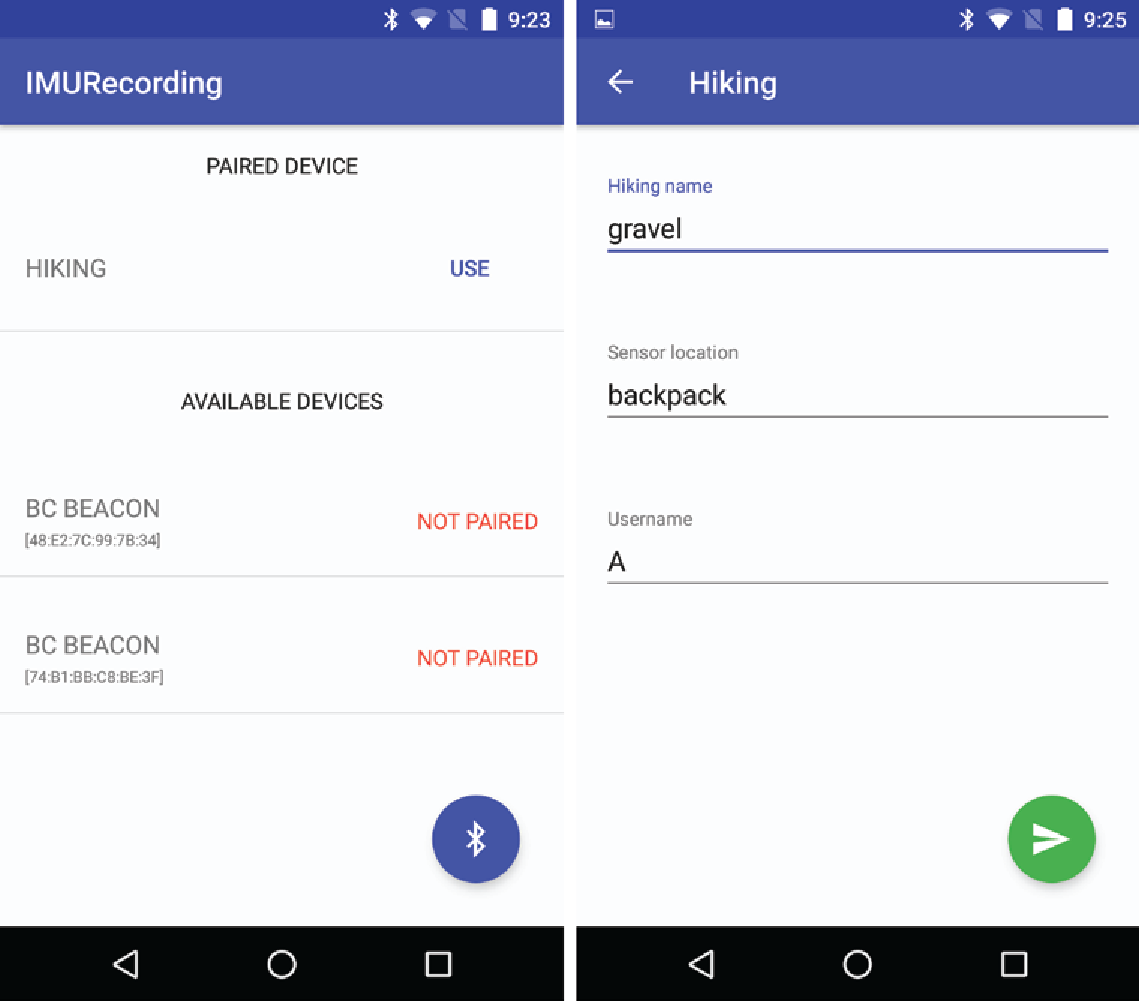
\includegraphics[width=.7\linewidth]{chapter4/application.pdf}
        \caption[Captures d'écran de l'application \textit{Android} exécutée sur \texttt{cell\_oper} qui a permis le pilotage et l'étiquetage des données brutes.]{Captures d'écrans de l'application \textit{Android} exécutée sur \texttt{cell\_oper} qui a permis de le pilotage et l'étiquetage les données brutes \citep{Thullier2017}.}
	\label{fig:application}
\end{figure}

Par ailleurs, le fonctionnement de la seconde application\footnote{\url{https://github.com/FlorentinTh/SoilTypesRecognition-AndroidAppRecording}} \textit{Android} qui a été développée demeure identique à celui du firmware du \textit{wearable device}. En effet, celle-ci reçoit par \acs{BLE} les mêmes informations de configuration envoyées par le biais de l'application qui s'exécute sur \texttt{cell\_oper}. De la même manière, les données inertielles (accéléromètre, gyroscope, magnétomètre) ainsi que les angles d'Euler sont enregistrés toutes les secondes sur la mémoire flash du téléphone sur lequel elle est exécutée (\texttt{cell}), au format \acs{CSV} et à une même fréquence stabilisée à 60 Hz.

\subsection{Procédure}
Pour effectuer la collecte de données, il était nécessaire que les expérimentations soient conduites dans des situations se rapprochant le plus possible de cas d'utilisation réels. En ce sens, trois emplacements ont été adoptés comme étant les plus probables d'être choisis par les utilisateurs du \textit{wearable device}. Le premier est à l'intérieur d'un sac porté sur les épaules grâce aux anses, comme un sac à main. La seconde possibilité identifiée pour le port du dispositif est à l'intérieur d'un sac à dos et enfin, le dernier positionnement est simplement à l'intérieur de la poche d'une veste. Cependant, puisque ce travail s'intéresse à déterminer avec précision l'impact de l'emplacement du \textit{wearable device} sur la reconnaissance des types de sols, il a été demandé aux participants de l'expérimentation de porter le dispositif à la fois sur l'épaule de droite et l'épaule de gauche pour le sac à main, tel qu'illustré par la figure \ref{fig:positions_a}. Aussi, celui-ci était lesté avec une masse supplémentaire d'un kilogramme. De la même manière, les participants ont été invités à porter le dispositif à l'intérieur des poches à droite et à gauche de la veste, comme montré par la figure \ref{fig:positions_b}, où une attention particulière a été portée sur le fait de conserver la veste fermée\textemdash ceci dans l'objectif de réduire le bruit potentiel induit sur les données inertielles par l'oscillation des bras lors de la marche. Finalement, en ce qui concerne le sac à dos, sa contenance était de $20\:L$ et il était lesté avec un poids supplémentaire de $3\:kg$. De plus, le \textit{wearable device} a été positionné dans la même poche du sac et dans la même direction pour tous les participants de l'expérimentation.

\begin{figure}[H]
	\centering
	\subfloat[Positionnement du \textit{wearable device} à l'intérieur d'un sac bandoulière porté sur les épaules de droite et de gauche.]{
		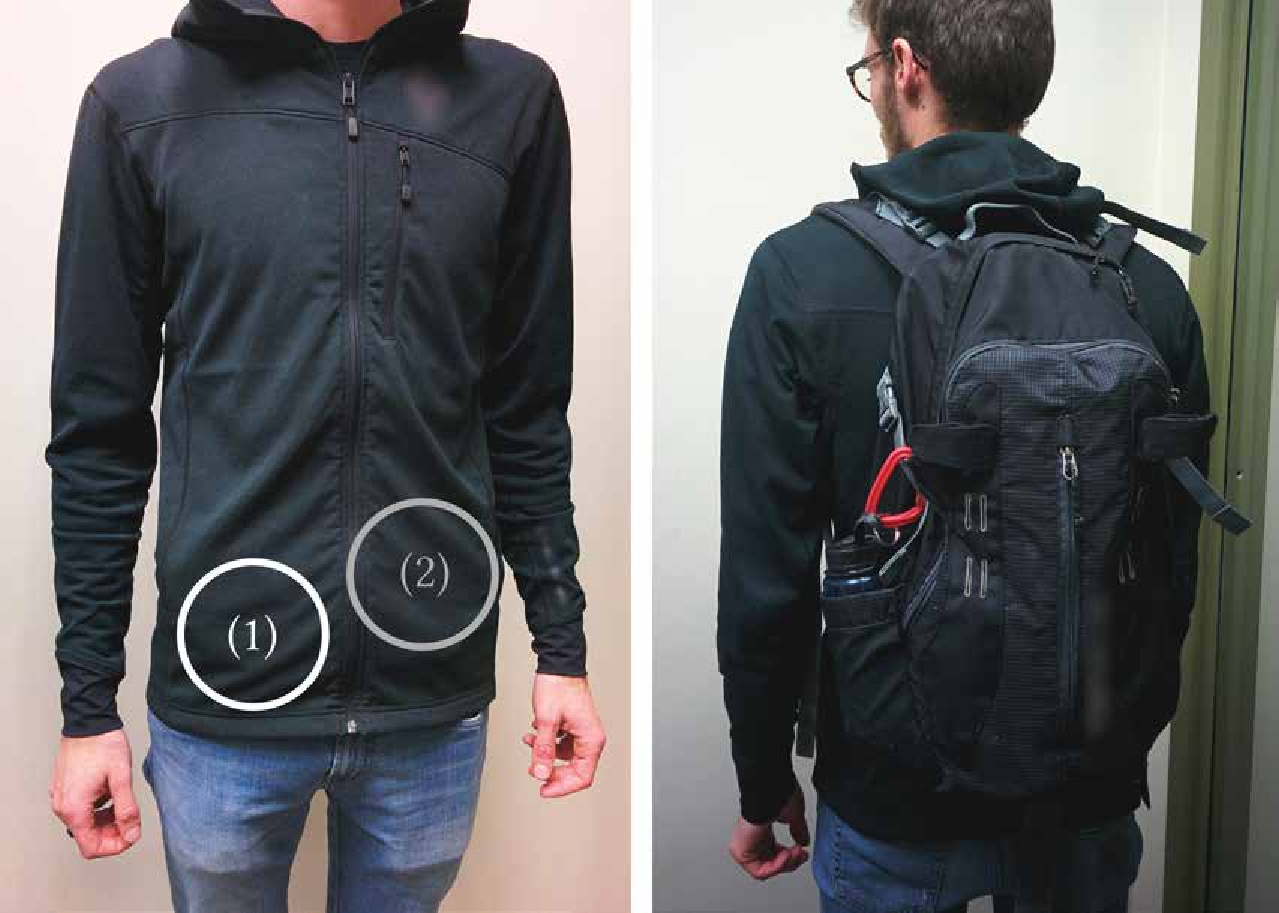
\includegraphics[width=.47\linewidth]{chapter4/positions_a.pdf}
		\label{fig:positions_a}
    }
	\hspace*{\fill}
	\subfloat[De gauche à droite, positionnement du \textit{wearable device} dans les poches de droite (1) et de gauche (2) ainsi qu'à l'intérieur d'un sac à dos ordinaire de $20\:L$.]{
		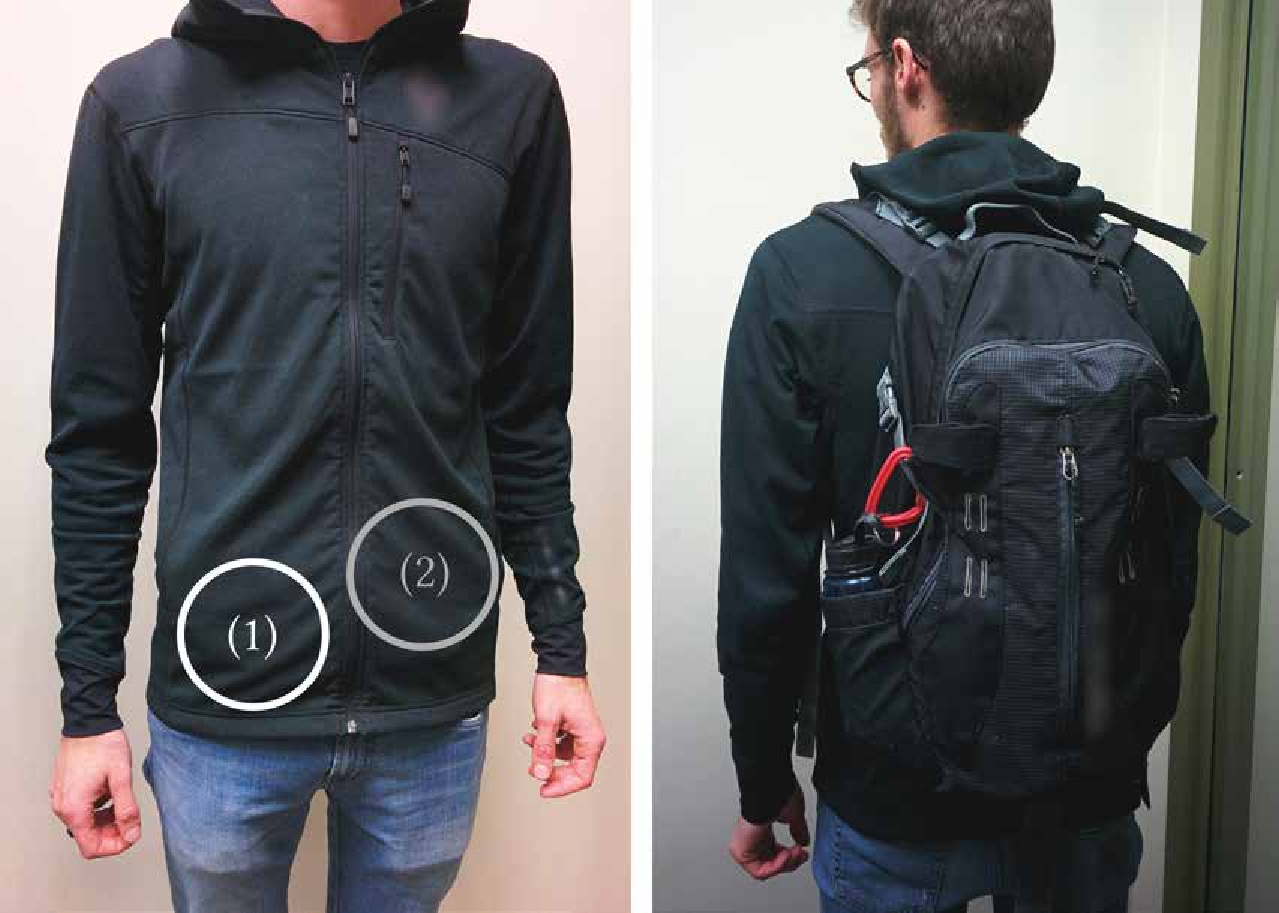
\includegraphics[width=.48\linewidth]{chapter4/positions_b.pdf}
		\label{fig:positions_b}
    }
    \caption[Les cinq emplacements où le \textit{wearable device} a été positionné pendant l'expérimentation.]{Les cinq emplacements où le \textit{wearable device} a été positionné pendant l'expérimentation \citep{Thullier2017}.}
    \label{fig:positions}
\end{figure}

Dès lors que les instructions au sujet du positionnement du dispositif ont été présentées aux participants, ils ont été invités à effectuer six allers-retours sur chaque type de sol, pour chaque position donnée. Un superviseur en charge de la gestion du \textit{wearable device} par l'intermédiaire de l'application \textit{Android} dédiée leur a indiqué, à la fois quand commencer et quand s'arrêter de marcher. Tout d'abord, il leur a été demandé de commencer par les graviers placés à l'intérieur du bac décrit précédemment. Dans un second temps, ils ont été invités à effectuer la même opération sur le sol à côté du bac, considéré comme étant une sorte de ciment. Les participants ont ensuite été sollicités à sortir pour effectuer six autres allers et retours dans la neige. Afin de rester cohérents avec la procédure de l'expérimentation réalisée au sein du laboratoire, un ruban à mesurer respectant la longueur du bac a été placé sur la neige pour indiquer aux participants où faire demie tour. Enfin, puisque les graviers à l'intérieur du bac devaient être remplacés, les participants ont été recontactés pour effectuer ultérieurement l'expérimentation sur le sable. Cette même procédure a été répétée aussi bien avec la version 2 du \textit{wearable device} (\texttt{wear\_v2}), ainsi qu'avec le téléphone intelligent (\texttt{cell}) à l'exception faite des enregistrements récoltés sur la neige, puisque la période de l'année durant laquelle cette deuxième partie de l'expérimentation a été conduite ne le permettait pas.

\section{Résultats et discussion}

\subsection{Ensembles de données}

Afin de valider que la méthode de reconnaissance des types de sols proposée dans ce premier travail demeure suffisamment précise et fiable, il a été nécessaire de produire plusieurs jeux de données composés des caractéristiques discriminantes et des informations de configuration qui constituent l'étiquetage des données. L'ensemble des différents jeux de données utilisés dans ces expérimentations sont disponibles en \textit{open source}\footnote{\url{https://github.com/LIARALab/Datasets/tree/master/SoilTypesRecognition}} et la liste de ceux-ci est fournie par le tableau \ref{tab:datasets}.

Puisque les expérimentations faites par les participants ont permis l'échantillonnage de données brutes à une fréquence stabilisée à 60 Hz, il a tout d'abord été nécessaire de définir la taille de la fenêtre pour réaliser le calcul des caractéristiques discriminantes. Celle-ci a été déterminée de manière empirique selon le temps moyen pour marcher la distance d'un aller-retour dans le bac qui a été observé pour chaque participant. Ainsi, puisque la moyenne de ces temps a été de 6 secondes, c'est ce découpage qui a été utilisé pour procéder au calcul des caractéristiques discriminantes, soit une fenêtre de taille $6\:s \times 60\:Hz = 360$ instances de données brutes pour chaque participant, sur chaque type de sol et pour chaque position. Finalement, ces jeux de données ont été utilisés en entrée des algorithmes d'apprentissage pour la reconnaissance des types de sols.

\begin{table}[H]
	\caption{Liste détaillée des ensembles de données produits, où les noms sont exprimés avec la notation \acs{BNF}.}
	\label{tab:datasets}
	\begin{center}
		\resizebox{.9\textwidth}{!}{%
			\begin{tabular}{@{}rl@{}}
				\toprule
				\textbf{Jeu de données} & \textbf{Description} \\ \midrule
				\texttt{soil\_type\_}\texttt{[ }\texttt{wear\_v1}\texttt{ | }\texttt{wear\_v2}\texttt{ | }\texttt{cell}\texttt{ ]}\_\texttt{[ }\texttt{6}\texttt{ | }\texttt{9}\texttt{ | }\texttt{12}\texttt{ ]} & \begin{tabular}[c]{@{}l@{}}Chaque instance est étiquetée \\[-15pt] avec le type de sol correspondant \\[-15pt] (\textit{p. ex.} \texttt{sable}).\end{tabular} \\
				\texttt{soil\_type\_position\_}\texttt{[ }\texttt{wear\_v1}\texttt{ | }\texttt{wear\_v2}\texttt{ | }\texttt{cell}\texttt{ ]}\_\texttt{[ }\texttt{6}\texttt{ | }\texttt{9}\texttt{ | }\texttt{12}\texttt{ ]} & \begin{tabular}[c]{@{}l@{}}Chaque instance est étiquetée avec le type de sol \\[-15pt] correspondant et la position du wearable device \\[-15pt] (\textit{p. ex.} \texttt{poche\_droite\_sable}).\end{tabular} \\ \bottomrule
			\end{tabular}%
		}
	\end{center}
\end{table}

D'autre part, pour vérifier l'hypothèse d'indépendance de positionnement, c'est-à-dire, la capacité pour le système à reconnaitre les types de sols qu'importe l'emplacement du \textit{wearable device}, des ensembles de données distincts ont été produits pour chaque positionnement et dont les données sont étiquetées avec le type de sol uniquement.

\subsection{Évaluation de la performance}

La performance de la méthode pour la reconnaissance des types de sols proposée dans ce chapitre a été évaluée selon plusieurs méthodes d'apprentissage. Celles-ci ont été réalisées grâce au \textit{workbench} d'apprentissage machine \acs{WEKA} (\acl{WEKA}) \citep{Holmes1994} qui a été employé en tant que librairie dans une application\footnote{\url{https://github.com/FlorentinTh/SoilTypesDetection}} de type \ac{CLI} développée en Java. Ainsi, l'évaluation de la performance de la reconnaissance a été déterminée selon la validation croisée en $k$-plis, par le biais de cette application.

La méthode de la validation croisée en $k$-plis est très largement utilisée dans la littérature de l'apprentissage machine au sens large \citep{Vail2004, Arlot2010, Kertesz2016}. En effet, l'avantage principal de cette technique est qu'elle permet l'utilisation de l'intégralité des données disponibles aussi bien pour la phase d'entraînement que pour la reconnaissance. De plus, celle-ci va permettre de minimiser le biais potentiel d'un ensemble de données de validation construit de manière empirique, c'est-à-dire, réduire les problèmes liés à une mauvaise distribution de ces données comme le sur-apprentissage.

Le fonctionnement de la validation croisée en $k$-plis est relativement simple. Prenons par exemple un ensemble de données binaires (\og $+$ \fg et \og $-$ \fg) sur lequel on souhaite mettre en place un système de reconnaissance grâce à un algorithme d'apprentissage dont la performance est évaluée avec une validation croisée où $k=3$. La première étape consiste à découper cet ensemble de données en trois plis mutuellement disjoints. Néanmoins, puisque les données dans l'ensemble initial ne sont pas triées, il est important de s'assurer, lors du découpage, que les instances étiquetées soit par un \og $+$ \fg soit par un \og $-$ \fg soient réparties selon la même fréquence dans les trois plis. C'est le principe de la stratification des données. Dans cet exemple, les trois plis sont notés $A$, $B$ et $C$, tel qu'illustré par la figure \ref{fig:cross_validation}. La deuxième étape de ce processus est d'entraîner une première fois l'algorithme d'apprentissage avec l'ensemble $B\cup C$ et d'évaluer la performance de la reconnaissance avec $A$. Cette mesure est notée $E_A$. Ensuite, cette étape est répétée pour les deux plis restant en utilisant les ensembles $A\cup C$ puis $A\cup B$ pour l'entraînement et respectivement $B$ puis $C$ pour quantifier la performance de la reconnaissance, ce qui permet alors d'obtenir $E_B$ et $E_C$. Enfin, la performance globale de la reconnaissance ($E$), est estimée par la moyenne des mesures obtenues pour chaque pli.

\begin{figure}[H]
	\centering
	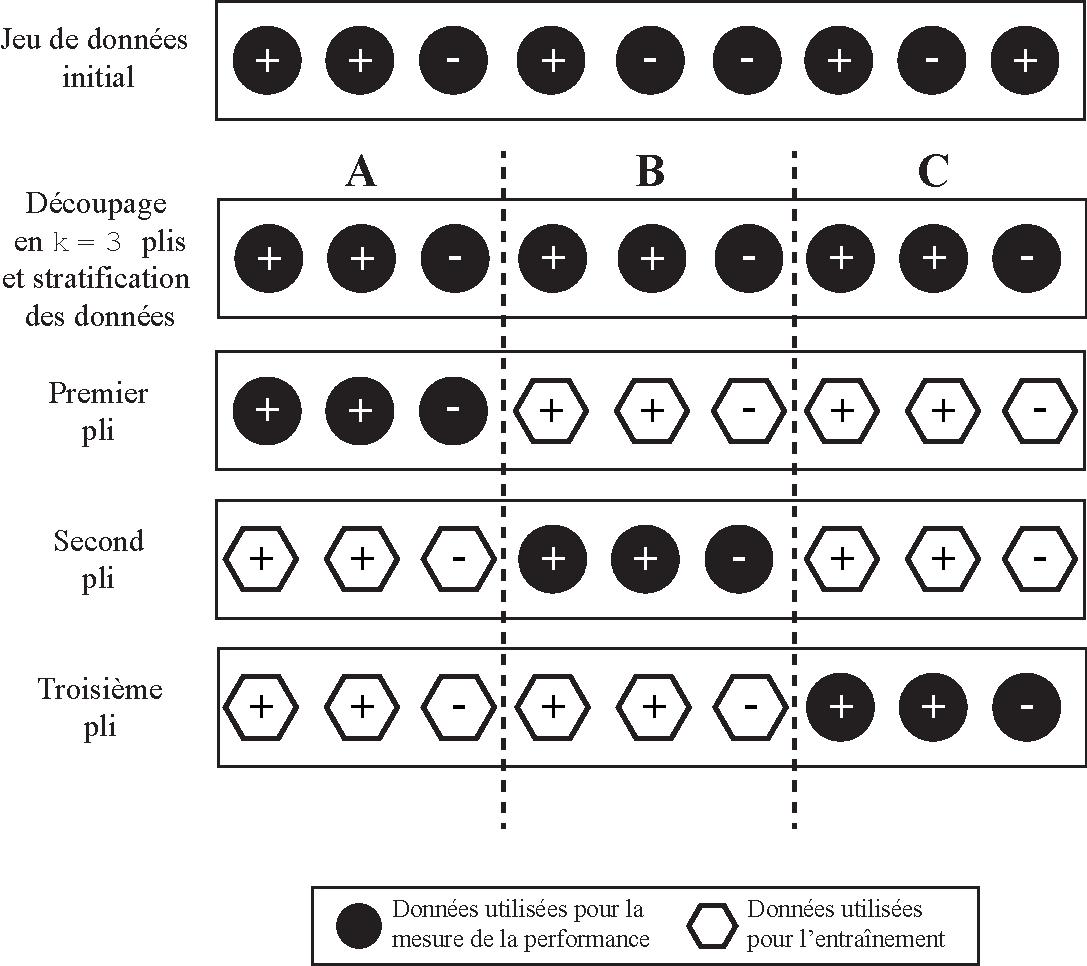
\includegraphics[width=.7\linewidth]{chapter4/cross_validation.pdf}
        \caption{Exemple d'une validation croisée où $k=3$ plis sur des données binaires.}
	\label{fig:cross_validation}
\end{figure}

Depuis l'apparition de l'apprentissage machine, de nombreux travaux ce sont concentrés sur l'optimisation de l'évaluation de la performance de ces systèmes \citep{Witten2016}. Ainsi, le nombre de plis à utiliser dans une validation croisée admis comme standard aujourd'hui est $k=10$. De ce fait, pour que l'évaluation du système proposé dans ce chapitre demeure cohérente avec celles définies dans la littérature, une validation croisée en 10 plis a donc été retenue.

\subsection{Résultats obtenus}

\subsubsection{\textit{Version 1 du wearable device}}

Dans un premier temps, la performance du système de reconnaissance des types de sols a été évaluée sur les données obtenues avec la version 1 du \textit{wearable device}. Pour ce faire, plusieurs modèles d'apprentissage ont été construits en utilisant différents paramètres pour l'algorithme \textit{random forest}. Puisqu'il est préférable qu'une forêt d'arbres décisionnels soit composée d'un grand nombre d'arbres \citep{Breiman2001}, les deux valeurs : $B=150$ et $B=300$ arbres ont été comparées\textemdash ceci dans le but de répondre aux exigences proposées par \cite{Breiman2001}, ainsi que pour conserver un temps de calcul acceptable. En ce qui concerne le paramètre relatif au nombre de variables aléatoires ($F$), les trois valeurs préconisées dans la littérature, soit $F_0=\lfloor \frac{1}{2}\sqrt{m}\rfloor$, $F_1=\lfloor log_2(m) + 1\rfloor$ et $F_2=\lfloor \sqrt{m}\rfloor$ ont également été comparées. Enfin, de par l'implémentation utilisée dans ce système, la fonction employée pour mesurer la qualité de la division des n\oe{}uds de l'arbre ($C$) demeure l'évaluation du gain en information basé sur l'entropie de Shannon, pour chaque expérimentation. La figure \ref{fig:results_wear_v1_rf} montre une représentation graphique des résultats obtenus pour chaque paramétrage de l'algorithme \textit{random forest}, évalué sur les deux ensembles de données.

De la même manière, la performance de l'algorithme des $k$ plus proches voisins a été évaluée afin que les résultats puissent être comparés avec ceux obtenus pour l'algorithme \textit{random forest}. Pour ce faire, les mesures de la distance euclidienne ($D_e$) ainsi que de la distance de Manhattan ($D_m$) ont toutes deux été utilisées. Afin de déterminer le nombre de voisins ($k$) optimal pour ce système de reconnaissance, toutes les valeurs comprises entre $k=1$ et $k=\sqrt{m}$, où $m$ correspond au nombre de caractéristiques discriminantes, ont été essayées et les résultats obtenus ont été comparés de manière empirique. \hl{Étonnamment, il est apparu que le nombre approprié de voisins à considérer était d'un seul, bien que celui-ci demeure la borne inférieure de l'ensemble des possibilités qu'il est généralement conseillé d'éviter afin de ne pas courir le risque de se retrouver avec un modèle en sur-apprentissage} \citep{Duda2000}\hl{. Néanmoins, puisque des résultats similaires ont été observés pour} $k=3$\hl{, cette observation suggère alors qu'au sein de l'espace vectoriel, une majorité des données inertielles sont bien séparées en différents groupes distincts selon les étiquettes attribuées à chacune d'entre elles. Par conséquent, l'utilisation de} $k=1$ \hl{a été préférée afin de minimiser l'impact de cette opération sur les performances du \textit{wearable device}}. La figure \ref{fig:results_wear_v1_knn} montre une représentation graphique des résultats obtenus pour chaque paramétrage de l'algorithme \acs{KNN}, évalué grâce à une recherche linéaire du plus proche voisin pour les deux jeux de données. Par ailleurs, l'ensemble des résultats de cette première expérimentation est fourni en détail, pour les deux algorithmes, dans l'annexe \ref{anx:a1}.

En s'appuyant sur ces résultats, il est possible d'affirmer que les paramètres optimaux qui sont suggérés pour la méthode de reconnaissance des types de sols, lorsqu'elle est réalisée avec l'algorithme \textit{random forest} sont : $B=300$ arbres et un nombre de variables aléatoires équivalent à $F_1=\log_2(m) + 1$, où $m$ correspond au nombre de caractéristiques discriminantes. En effet, c'est avec ces paramètres que les meilleurs résultats ont été observés, c'est-à-dire, une $F\mbox{-}mesure$ moyenne des deux jeux de données de $86\%$. De plus, la même $F\mbox{-}mesure$ moyenne a été obtenue avec l'algorithme \acs{KNN} lorsque celui-ci est configuré avec la fonction de distance de Manhattan. En comparaison, l'emploi de la fonction de distance euclidienne a, quant à elle, montré de moins bons résultats. De ce fait, la mesure de distance qui semble la plus optimale pour cet algorithme est donc $D_m$.

\begin{figure}[H]
    \centering
	\subfloat[Les $F\mbox{-} mesures$ obtenues sur les deux ensembles de données avec les différentes configurations pour l'algorithme \textit{random forest}.]{
		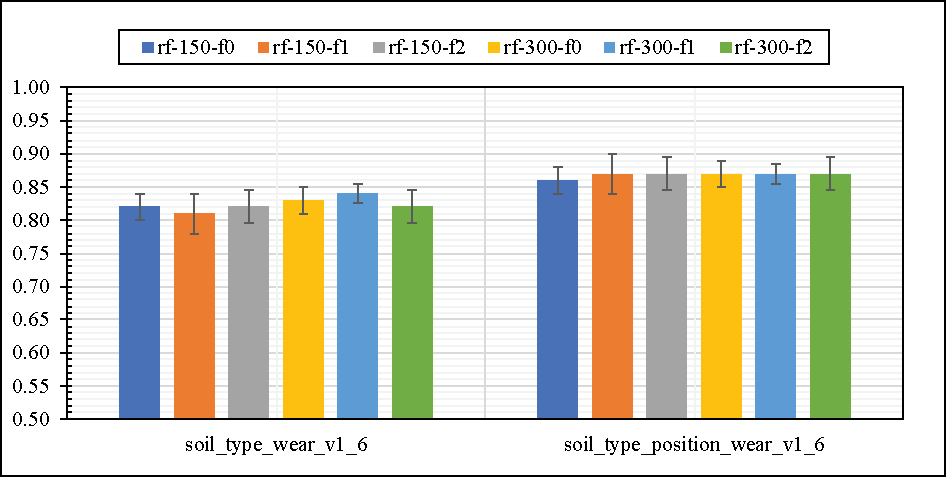
\includegraphics[width=.7\linewidth]{chapter4/results_wear_v1_rf.pdf}
		\label{fig:results_wear_v1_rf}
    }
    \\[20pt]
	\subfloat[Les $F\mbox{-} mesures$ obtenues sur les deux ensembles de données avec les différentes configurations pour l'algorithme des $k$ plus proches voisins.]{
		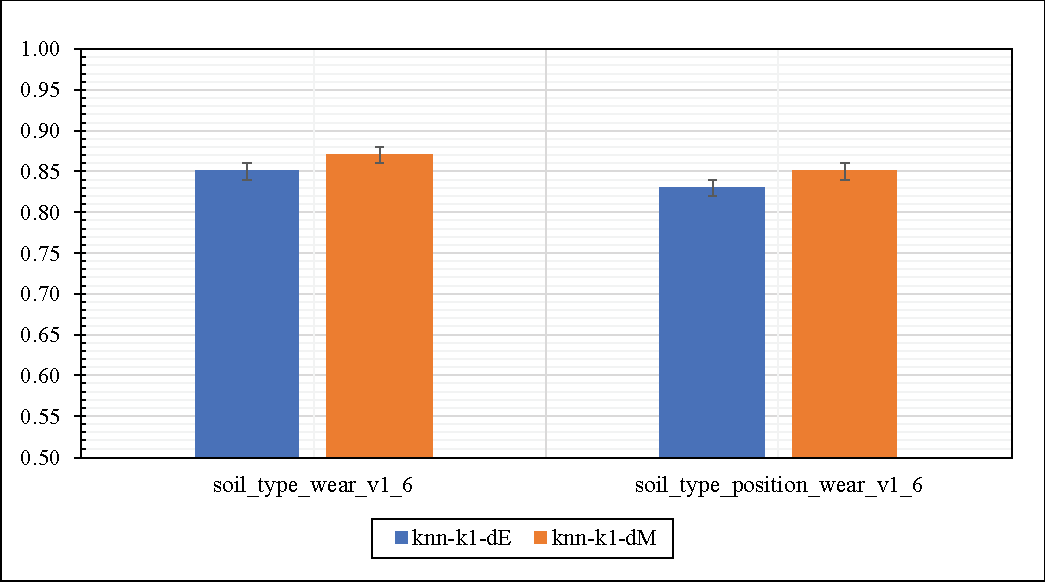
\includegraphics[width=.7\linewidth]{chapter4/results_wear_v1_knn.pdf}
		\label{fig:results_wear_v1_knn}
    }
    \caption[Les $F\mbox{-} mesures$ obtenues sur les deux ensembles de données avec les différentes configurations pour les algorithmes \textit{random forest} et \acs{KNN} avec la version 1 du \textit{wearable device}.]{Les $F\mbox{-} mesures$ obtenues sur les deux ensembles de données avec les différentes configurations pour les algorithmes \textit{random forest} et \acs{KNN} avec la version 1 du \textit{wearable device} \citep{Thullier2017}.}
    \label{fig:results_wear_v1}
\end{figure}

Afin de s'assurer que la reconnaissance des sols soit fonctionnelle, et ce, indépendamment de la position choisie par l'utilisateur pour le porter, cinq jeux de données distincts ont été construits à partir des ensembles de données initiaux utilisés dans l'expérience précédente. Ainsi, ils constituent un ensemble de données par emplacement dont les étiquettes correspondent aux types de sols uniquement. Ensuite, l'évaluation de la performance de reconnaissance a été réalisée avec les deux mêmes algorithmes d'apprentissage, configurés avec les paramètres qui ont été déterminés optimaux dans l'expérimentation précédente. Les résultats obtenus sont données par les courbes continues représentées sur la figure \ref{fig:pos_ind_wear_v1}. De plus, afin de déterminer si la position du \textit{wearable device} avait un impact significatif sur le taux de reconnaissance, la moyenne des $F\mbox{-}mesures$ obtenues pour chaque position par rapport aux types de sols a été évaluée à l'aide du jeu de données \og \texttt{soil\_type\_position\_wear\_v1\_6} \fg. Ce sont les courbes discontinues également représentés sur la figure \ref{fig:pos_ind_wear_v1}. Celles-ci déterminent alors les valeurs de référence pour chaque position.

L'expression graphique donnée par ses différentes courbes permet de constater qu'aucune position distincte du \textit{wearable device} n'a un impact significatif sur la performance de la reconnaissance des types de sols. En effet, les différences maximum observées dans les $F\mbox{-}mesures$ sont de $2\%$ et $6\%$, respectivement avec l'algorithme \textit{random forest} et \acs{KNN}. De plus, il est possible, pour chaque algorithme, d'observer une similarité entre la tendance de la courbe exprimant les résultats et la courbe de référence.

\begin{figure}[H]
  \centering
\subfloat[Les $F\mbox{-} mesures$ obtenues pour chaque position lors de l'évaluation de l'indépendance de positionnement avec l'algorithme \textit{random forest}, où $B=300$ et $F=F_1$.]{
  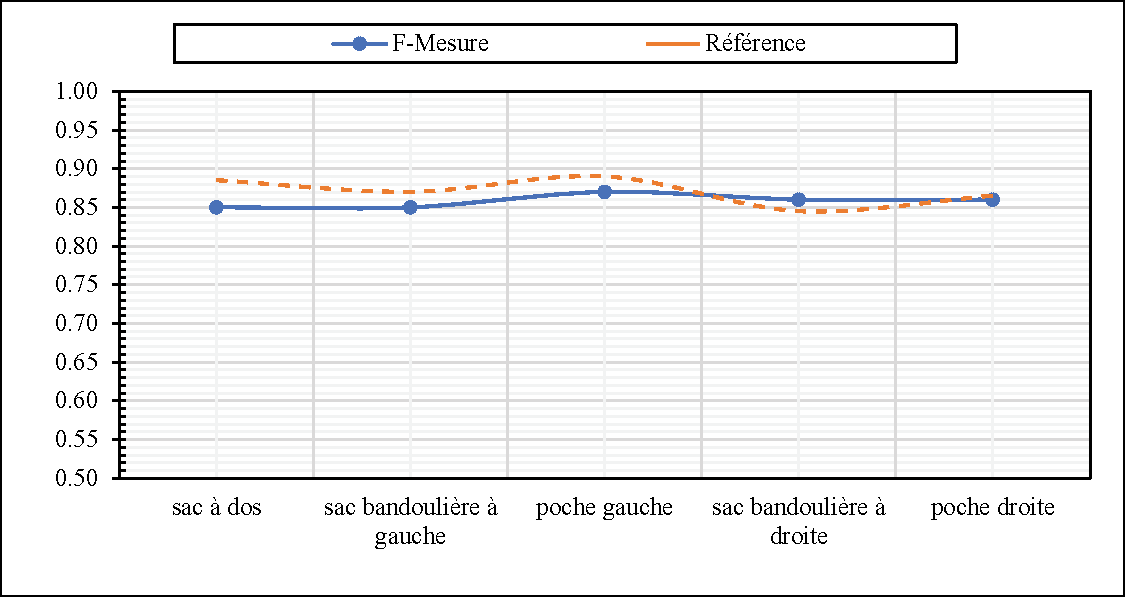
\includegraphics[width=.7\linewidth]{chapter4/pos_ind_rf_wear_1.pdf}
  \label{fig:pos_ind_rf_wear_1}
  }
  \\[20pt]
\subfloat[Les $F\mbox{-} mesures$ obtenues pour chaque position lors de l'évaluation de l'indépendance de positionnement avec l'algorithme \acs{KNN} où la mesure de distance utilisée est $D_m$.]{
  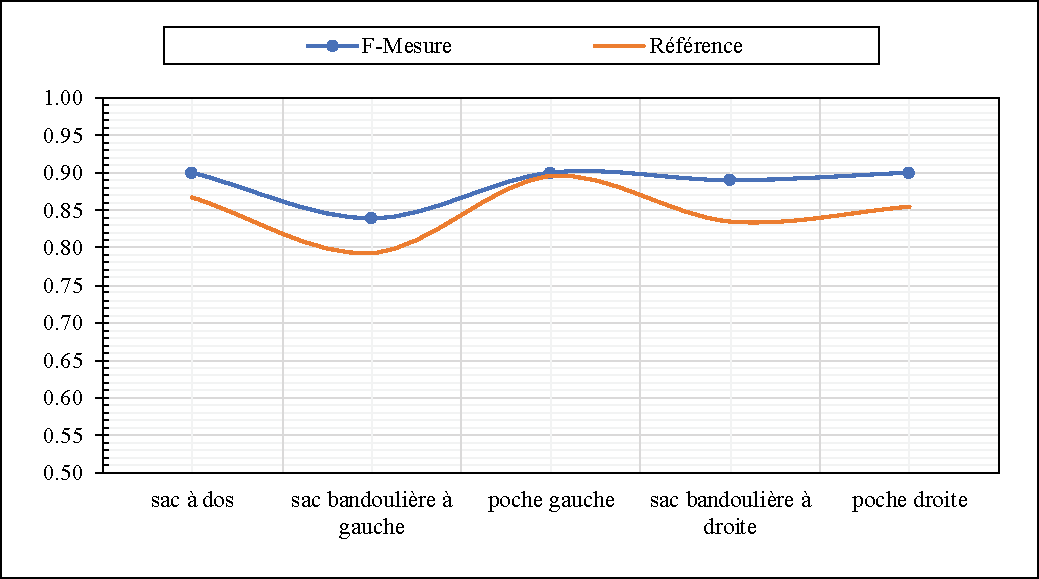
\includegraphics[width=.7\linewidth]{chapter4/pos_ind_knn_wear_1.pdf}
  \label{fig:pos_ind_knn_wear_1}
  }
  \caption[Les $F\mbox{-} mesures$ pour chaque position par rapport aux valeurs références permettant l'évaluation de l'indépendance de positionnement du \textit{wearable device} dans sa version 1, pour les deux algorithmes : \textit{random forest} et \acs{KNN}.]{Les $F\mbox{-} mesures$ pour chaque position par rapport aux valeurs références permettant l'évaluation de l'indépendance de positionnement du \textit{wearable device} dans sa version 1, pour les deux algorithmes : \textit{random forest} et \acs{KNN} \citep{Thullier2017}.}
  \label{fig:pos_ind_wear_v1}
\end{figure}


\subsubsection{\textit{Version 2 du wearable device}}

Dans un second temps, les deux expérimentations précédentes ont été reproduites selon la même procédure avec la version 2 du \textit{wearable device}. Puisque cette version offre un plus grand nombre d'axes pour la centrale inertielle, l'objectif était de vérifier l'impact des axes supplémentaires sur la reconnaissance des types de sols afin de proposer l'implémentation matérielle la plus précise possible pour le \textit{wearable device}. La figure \ref{fig:results_wear_v2} présente les résultats pour les deux algorithmes configurés avec les paramètres optimaux identifiés précédemment pour les deux jeux de données différents. Pour atténuer la perte d'information dans cette expérimentation comparativement à la première, les données de l'\acs{IMU} avec seulement 6 axes ont également été traitées.

\begin{figure}[H]
	\centering
	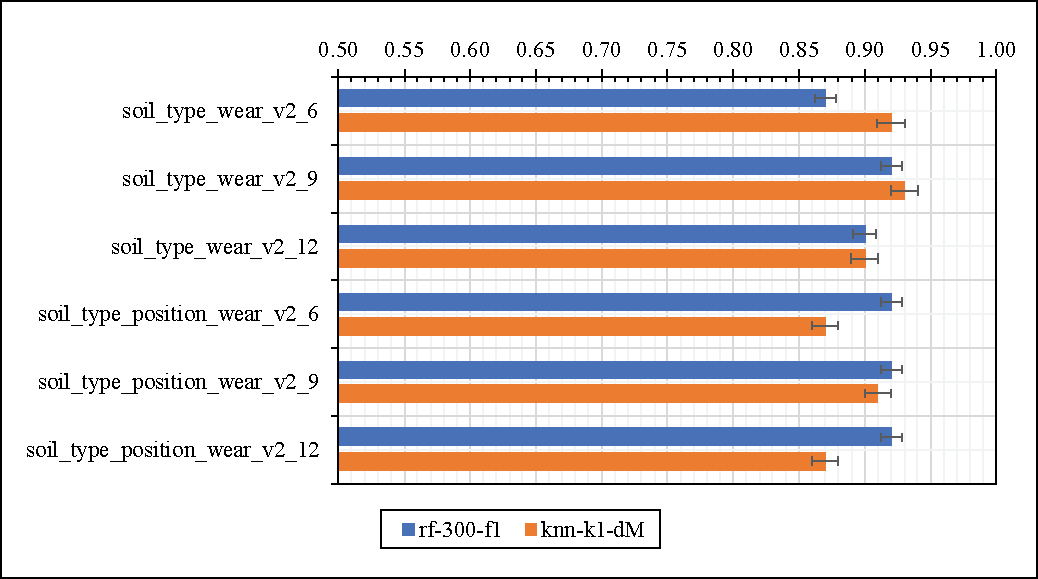
\includegraphics[width=.7\linewidth]{chapter4/results_wear_v2.pdf}
        \caption[Les $F\mbox{-} mesures$ obtenues sur les deux ensembles de données enregistrés avec la version 2 du \textit{wearable device} pour les algorithmes \textit{random forest} et \acs{KNN} configurés avec les paramètres optimaux.]{Les $F\mbox{-} mesures$ obtenues sur les deux ensembles de données enregistrés avec la version 2 du \textit{wearable device} pour les algorithmes \textit{random forest} et \acs{KNN} configurés avec les paramètres optimaux \citep{Thullier2017}.}
	\label{fig:results_wear_v2}
\end{figure}

Premièrement, ces résultats montrent que la perte d'information entre les expériences réalisées avec la première version du dispositif et la seconde n'ont pas un impact significatif sur la reconnaissance des types de sols. En effet, la même $F\mbox{-}mesure$ a été obtenue avec l'algorithme \textit{random forest}. Par ailleurs, la $F\mbox{-}mesure$ obtenue pour l'algorithme des $k$ plus proches voisins \hl{a, quant à elle, augmentée de 6\%.} De plus, le \texttt{LSM9DS1} est, en théorie, une centrale inertielle beaucoup plus précise que celle utilisée lors de l'expérimentation avec la version 1 du dispositif. \hl{En ce sens,} une amélioration de la reconnaissance a été constatée avec le jeu de données produit par l'\acs{IMU} 9-axes, tandis qu'une amélioration négligeable a été observée avec l'ensemble de données contenant les angles d'Euler. Enfin, les résultats détaillés fournis en annexe \ref{anx:a2}, permettent de confirmer que les paramètres utilisés dans la configuration des deux algorithmes pour cette expérimentation sont toujours les plus optimaux.

En ce qui concerne l'indépendance du positionnement du \textit{wearable device} dans sa seconde version, les mêmes observations peuvent être établies selon les résultats qui ont été obtenus. Ils sont exposés en figure \ref{fig:pos_ind_wear_v2}. En effet, les mêmes similarités sont visibles entre les tendances des courbes exprimant les résultats et celles de référence.

\begin{figure}[H]
    \centering
	\subfloat[Les $F\mbox{-} mesures$ obtenues pour l'évaluation de l'indépendance de positionnement avec l'algorithme \textit{random forest} configurés avec les paramètres optimaux.]{
		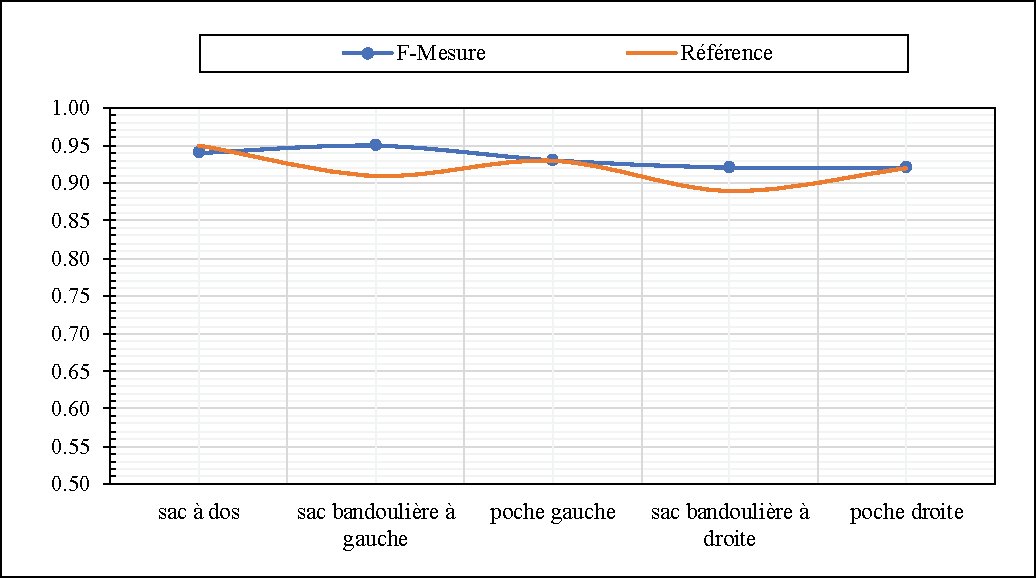
\includegraphics[width=.7\linewidth]{chapter4/pos_ind_rf_wear_2.pdf}
		\label{fig:pos_ind_rf_wear_2}
    }
    \\[20pt]
	\subfloat[Les $F\mbox{-} mesures$ obtenues pour l'évaluation de l'indépendance de positionnement avec l'algorithme \acs{KNN} configurés avec les paramètres optimaux.]{
		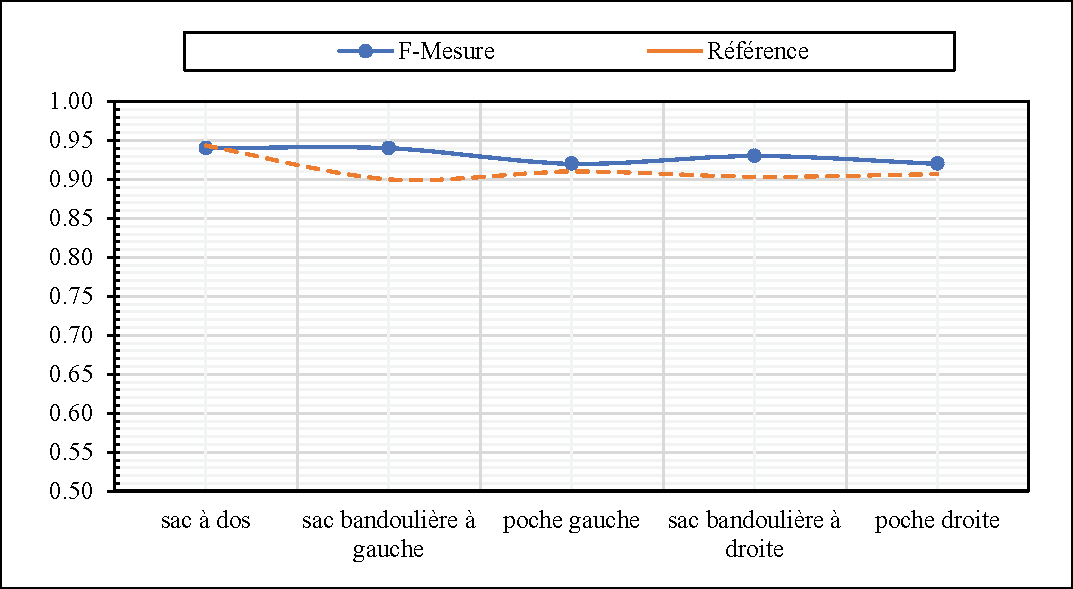
\includegraphics[width=.7\linewidth]{chapter4/pos_ind_knn_wear_2.pdf}
		\label{fig:pos_ind_knn_wear_2}
    }
    \caption[Les $F\mbox{-} mesures$ obtenues par rapport aux valeurs de référence permettant l'évaluation de l'indépendance de positionnement du \textit{wearable device} dans sa version 2, pour les deux algorithmes : \textit{random forest} et \acs{KNN} configurés avec les paramètres optimaux.]{Les $F\mbox{-} mesures$ obtenues par rapport aux valeurs de référence permettant l'évaluation de l'indépendance de positionnement du \textit{wearable device} dans sa version 2, pour les deux algorithmes : \textit{random forest} et \acs{KNN} configurés avec les paramètres optimaux \citep{Thullier2017}.}
    \label{fig:pos_ind_wear_v2}
\end{figure}

\subsubsection{\textit{Téléphone intelligent}}

En dernier lieu, l'analyse de la performance de la reconnaissance des types de sols a été reproduite selon la même procédure, en utilisant un téléphone intelligent. Les résultats obtenus avec les paramètres optimaux pour les deux algorithmes sont illustrés en figure \ref{fig:results_cell}. Néanmoins, l'annexe \ref{anx:a3} présente de façon plus précise l'ensemble des résultats acquis pour tous les jeux de données et toutes les configurations possibles pour les algorithmes de reconnaissance. Ces résultats montrent une excellente performance de reconnaissance globale. Bien que ces résultats demeurent principalement comparables à ceux obtenus avec le \textit{wearable device}, le taux de reconnaissance, dans cette configuration, ne semble pas affecté ni par le nombre d'axes admis par la centrale inertielle, ni par l'algorithme de reconnaissance et ses paramètres.

\begin{figure}[H]
	\centering
	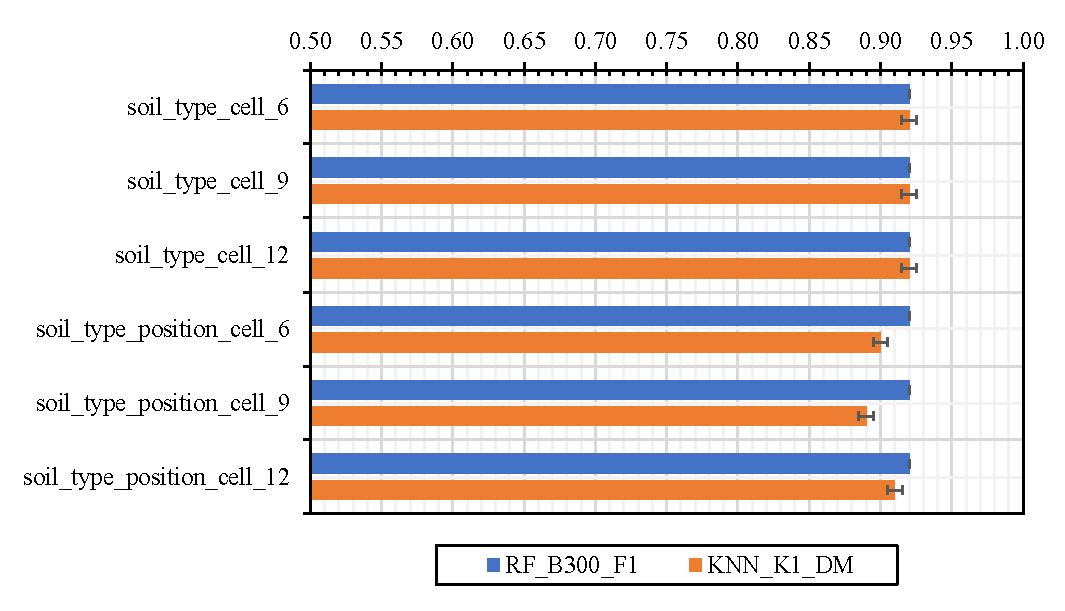
\includegraphics[width=.7\linewidth]{chapter4/results_cell.pdf}
        \caption[Les $F\mbox{-} mesures$ obtenues sur les deux ensembles de données enregistrés avec le téléphone intelligent pour les algorithmes \textit{random forest} et \acs{KNN} configurés avec les paramètres optimaux.]{Les $F\mbox{-} mesures$ obtenues sur les deux ensembles de données enregistrés avec le téléphone intelligent pour les algorithmes \textit{random forest} et \acs{KNN} configurés avec les paramètres optimaux \citep{Thullier2017}.}
	\label{fig:results_cell}
\end{figure}

\subsection{Discussion des résultats obtenus}

Dans la section précédente, l'ensemble des résultats ont été présentés sous forme de synthèse. Ceux-ci se sont révélés particulièrement précis dans la globalité des expérimentations qui ont été menées, sachant que les données inertielles sont parmi les données qui demeurent les plus sensibles au bruit. En effet, avec la première version du \textit{wearable device}, une performance de 86\% a été obtenue au meilleur des cas. Par ailleurs, il a été constaté que la version améliorée du dispositif (version 2) a permis une amélioration de 6\% des résultats de la reconnaissance des sols\textemdash soit une performance globale de 92\% en meilleur cas et en utilisant une centrale inertielle à 9-axes au lieu de 6-axes. Néanmoins, considérant le temps supplémentaire requis pour le traitement des angles d'Euler et la plus faible performance de reconnaissance obtenue dans cette configuration, il est possible d'affirmer que l'utilisation d'un \acs{IMU} 9-axes demeure la configuration matérielle idéale pour réaliser la reconnaissance des types de sols. Une telle différence entre les deux versions des dispositifs peut s'expliquer simplement par le fait que l'\acs{IMU} 6-axes directement intégré dans l'\textit{Arduino 101} est de moins bonne qualité et offre une moins bonne précision que le \texttt{LSM9DS1}.

Par ailleurs, les résultats obtenus avec le téléphone intelligent ont démontré une légère amélioration de la performance de reconnaissance globale. De plus, cette expérimentation a dévoilé une certaine stabilité dans les résultats obtenus malgré les différentes configurations qui ont été appliquées. L'hypothèse qui est formulée pour expliquer cet effet questionne la mise en place automatique d'un filtre sur les données issues du capteur inertiel (\textit{p. ex.} un filtre passe-bas). Il est en effet possible que le système d'exploitation applique un tel filtre avant que les données soient transmises à notre application. Par conséquent, cela implique que les données exploitées dans cette expérimentation ne sont pas exactement les données brutes et donc, qu'elles incluent beaucoup moins de bruit que les données produites par notre dispositif.

Par ailleurs, en ce qui concerne l'hypothèse de l'indépendance de la position du \textit{wearable device}, les comparaisons qui ont été effectuées ont montré que la position du dispositif n'impactait pas la performance de la reconnaissance des sols. Cependant, puisque les expérimentations ont impliqué un nombre relativement réduit de personnes, il apparaît pertinent d'en réaliser de nouvelles incluant un nombre beaucoup plus important de participants dans le but de renforcer cette affirmation.

Finalement, bien que l'ensemble des résultats obtenus soient très satisfaisants, nous pensons qu'il est encore possible de les améliorer. En effet, il serait envisageable de proposer une étape de prétraitement des données brutes afin d'en affiner la qualité. Cette étape pourrait, par exemple, constituer l'application de techniques telles qu'un filtre passe-bas ou un filtre de Kalman. De plus, il est possible que certaines caractéristiques proposées dans notre système ne soient pas suffisamment discriminantes et pourraient donc être supprimées. Par conséquent, cela permettrait principalement de réduire la dimension de nos ensembles de données. Ces deux possibilités d'amélioration pour notre système peuvent donc potentiellement aboutir à une meilleure performance de la reconnaissance des types de sols.

\section{Conclusion}

Dans ce chapitre, une nouvelle méthode pour reconnaitre les types de sols grâce aux données inertielles produites par la démarche humaine a été introduite. Pour ce faire, un \textit{wearable device} a été conçu dans le but d'enregistrer les données inertielles générées par son porteur. Dans une première version, ces données ont été obtenues par le biais d'un \acs{IMU} 6-axes déjà intégré au système électronique sur lequel notre choix s'est porté, c'est-à-dire, un \textit{Arduino 101}. Dans une seconde version, un \acs{IMU} 9-axes, plus précis, a été utilisé. L'enregistrement des données a été effectué grâce à une application \textit{Android}. Cette dernière était en charge de récupérer et d'étiqueter les données inertielles \textit{via} une connexion Bluetooth préalablement établie.

L'évaluation de cette méthode a été réalisée selon plusieurs expérimentations, toutes basées sur plusieurs étapes. La première concerne l'extraction de caractéristiques temporelles et fréquentielles sur les données brutes récoltées. Ensuite, les deux algorithmes d'apprentissage machine \textit{random forest} et des $k$ plus proches voisins ont été comparés. Enfin, la performance de la reconnaissance a pu être évaluée dans une dernière étape grâce au calcul de la $F\mbox{-} mesure$ réalisée par le biais de la méthode de la validation croisée en 10-plis. La première expérimentation s'est déroulée avec l'implication de neuf participants à qui il a été demandé de marcher sur quatre différents types de sols (\texttt{ciment}, \texttt{gravier}, \texttt{neige} et \texttt{sable}) en portant le \textit{wearable device} selon cinq positions distinctes. Bien que ces types de sols ne se retrouvent pas dans les habitats intelligents, ils ont été utilisés dans le protocole expérimental, car ceux-ci admettent des différences suffisamment importantes qui ont ainsi permis de valider la faisabilité de la méthode. Par conséquent, la seconde expérimentation a repris les mêmes grandes lignes du protocole de la première expérimentation à l'exception faite qu'un téléphone intelligent ait été ajouté en plus du dispositif pour l'enregistrement des données inertielles. De plus, puisque celle-ci s'est déroulée en été, il a été impossible d'établir une récolte de données sur la neige. Aussi, certains participants ayant quitté le laboratoire entre temps, cette expérimentation n'a impliquée que six participants parmi les neuf qui étaient présents lors de la première.

Les résultats obtenus grâce à ces expérimentations ont, dans un premier temps, permis de déterminer les paramètres optimaux à utiliser dans la configuration des algorithmes d'apprentissage machine. De plus, les différentes évaluations de la performance de reconnaissance ont montré une excellente précision, soit 86\% au mieux pour la première expérimentation et 92\% au mieux pour la seconde. Cette amélioration a permis de déterminer qu'une centrale inertielle à 9-axes était la configuration matérielle à adopter pour proposer une reconnaissance la plus précise possible. Enfin, bien que ces expérimentations aient également permis de statuer que la position du \textit{wearable device} n'avait aucun impact sur la performance de la reconnaissance des sols, il a été identifié que cette affirmation doit être renforcée par d'autres analyses incluant un nombre plus important de participants.
